% One-page layout: (proof-)reading on display
%%%% \documentclass[11pt,oneside,a4paper]{book}
% Two-page layout: final printing
\documentclass[11pt,twoside,a4paper]{book}
%=-=-=-=-=-=-=-=-=-=-=-=--=%
% The user of this template may find useful to have an alternative to these 
% officially suggested packages:
\usepackage[czech, english]{babel}
\usepackage[T1]{fontenc} % pouzije EC fonty 
\usepackage[utf8]{inputenc}

%=-=-=-=-=-=-=-=-=-=-=-=--=%
% Depending on your particular TeX distribution and version of conversion tools 
% (dvips/dvipdf/ps2pdf), some (advanced | desperate) users may prefer to use 
% different settings.
% Please uncomment the following style and use your CSLaTeX (cslatex/pdfcslatex) 
% to process your work. Note however, this file is in UTF-8 and a conversion to 
% your native encoding may be required. Some settings below depend on babel 
% macros and should also be modified. See \selectlanguage \iflanguage.
%\usepackage{czech}  %%%%%\usepackage[T1]{czech} %%%%[IL2] [T1] [OT1]
%=-=-=-=-=-=-=-=-=-=-=-=--=%

%%%%%%%%%%%%%%%%%%%%%%%%%%%%%%%%%%%%%%%
% Styles required in your work follow %
%%%%%%%%%%%%%%%%%%%%%%%%%%%%%%%%%%%%%%%
\usepackage{graphicx}
%\usepackage{indentfirst} %1. odstavec jako v cestine.

\usepackage{k336_thesis_macros} % specialni makra pro formatovani DP a BP
 % \newcommand{\bfig}{\begin{figure}\begin{center}}
 % \newcommand{\efig}{\end{center}\end{figure}}
 % umoznuje pouzit prikaz \bfig namisto \begin{figure}\begin{center} atd.

\newcommand\TypeOfWork{Master's Thesis}   \typeout{Master's Thesis} 

\newcommand\StudProgram{Open Informatics}  %master program
\newcommand\StudBranch{Software Engineering}   % pro prgoram EaI mag. (dobihajici i strukt.)


%%%%%%%%%%%%%%%%%%%%%%%%%%%%%%%%%%%%%%%%%%%%
% Vyplnte nazev prace, autora a vedouciho
% Set up Work Title, Author and Supervisor
%%%%%%%%%%%%%%%%%%%%%%%%%%%%%%%%%%%%%%%%%%%%

\newcommand\WorkTitle{Design and implementation of online banking system for near future}
\newcommand\FirstandFamilyName{Bc. Jan Fajfr}
\newcommand\Supervisor{Olivier Roux, OCTO Technology}


% Pouzijete-li pdflatex, tak je prijemne, kdyz bude mit vase prace
% funkcni odkazy i v pdf formatu
\usepackage[
pdftitle={\WorkTitle},
pdfauthor={\FirstandFamilyName},
bookmarks=true,
colorlinks=true,
breaklinks=true,
urlcolor=red,
citecolor=blue,
linkcolor=blue,
unicode=true,
]
{hyperref}



% Extension posted by Petr Dlouhy in order for better sources reference (\cite{} command) especially in Czech.
% April 2010
% See comment over \thebibliography command for details.

\usepackage[square, numbers]{natbib}             % sazba pouzite literatury
%\usepackage{url}
%\DeclareUrlCommand\url{\def\UrlLeft{<}\def\UrlRight{>}\urlstyle{tt}}  %rm/sf/tt
%\renewcommand{\emph}[1]{\textsl{#1}}    % melo by byt kurziva nebo sklonene,
\let\oldUrl\url
\renewcommand\url[1]{<\texttt{\oldUrl{#1}}>}

\begin{document}
\selectlanguage{english} 

% prikaz \typeout vypise vyse uvedena nastaveni v prikazovem okne
% pro pohodlne ladeni prace


\iflanguage{czech}{
	 \typeout{************************************************}
	 \typeout{Zvoleny jazyk: cestina}
	 \typeout{Typ prace: \TypeOfWork}
	 \typeout{Studijni program: \StudProgram}
	 \typeout{Obor: \StudBranch}
	 \typeout{Jmeno: \FirstandFamilyName}
	 \typeout{Nazev prace: \WorkTitle}
	 \typeout{Vedouci prace: \Supervisor}
	 \typeout{***************************************************}
	 \newcommand\Department{Katedra počítačů}
	 \newcommand\Faculty{Fakulta elektrotechnická}
	 \newcommand\University{České vysoké učení technické v Praze}
	 \newcommand\labelSupervisor{Vedoucí práce}
	 \newcommand\labelStudProgram{Studijní program}
	 \newcommand\labelStudBranch{Obor}
}{
	 \typeout{************************************************}
	 \typeout{Language: english}
	 \typeout{Type of Work: \TypeOfWork}
	 \typeout{Study Program: \StudProgram}
	 \typeout{Study Branch: \StudBranch}
	 \typeout{Author: \FirstandFamilyName}
	 \typeout{Title: \WorkTitle}
	 \typeout{Supervisor: \Supervisor}
	 \typeout{***************************************************}
	 \newcommand\Department{Department of Computer Science and Engineering}
	 \newcommand\Faculty{Faculty of Electrical Engineering}
	 \newcommand\University{Czech Technical University in Prague}
	 \newcommand\labelSupervisor{Supervisor}
	 \newcommand\labelStudProgram{Study Programme} 
	 \newcommand\labelStudBranch{Field of Study}
}




%%%%%%%%%%%%%%%%%%%%%%%%%%    Poznamky ke kompletaci prace
% Nasledujici pasaz uzavrenou v {} ve sve praci samozrejme 
% zakomentujte nebo odstrante. 
% Ve vysledne svazane praci bude nahrazena skutecnym 
% oficialnim zadanim vasi prace.
{
\pagenumbering{roman} \cleardoublepage \thispagestyle{empty}
\chapter*{Na tomto místě bude oficiální zadání vaší práce}
\begin{itemize}
\item Toto zadání je podepsané děkanem a vedoucím katedry,
\item musíte si ho vyzvednout na studiijním oddělení Katedry počítačů na Karlově náměstí,
\item v jedné odevzdané práci bude originál tohoto zadání (originál zůstává po obhajobě na katedře),
\item ve druhé bude na stejném místě neověřená kopie tohoto dokumentu (tato se vám vrátí po obhajobě).
\end{itemize}
\newpage
}

%%%%%%%%%%%%%%%%%%%%%%%%%%    Titulni stranka / Title page 

\coverpagestarts

%%%%%%%%%%%%%%%%%%%%%%%%%%%    Podekovani / Acknowledgements 

\acknowledgements
\noindent
I would like to thank to OCTO Technology for giving me the possibility to work on innovative subject as well to all my colleagues who helped me during the work on the thesis. Specially I would like to thank to Olivier Roux for his advices during the development of the project.

%%%%%%%%%%%%%%%%%%%%%%%%%%%   Prohlaseni / Declaration 

\declaration{In Prague on January 1, 2012}


%%%%%%%%%%%%%%%%%%%%%%%%%%%%    Abstract 

\abstractpage
Since online banking services were introduced, banks have offered to clients transaction and account management functions and did not propose many innovations. However the situation is changing. Banks have to compete with third party companies and are forced to change the way online banking is offered.

This thesis describes the changes in online banking and banking in general. The aim is to identify, describe and analyze the innovative trends as well as to propose a technical solution for online banking, taking into account the innovations which have to be implemented.

The architecture of the proposed application is prepared for integration into existing information system. Emphasis has been put on modularity and testability of the application.

% abstrakt v cestine.
\vglue60mm

\noindent{\Huge \textbf{Abstrakt}}
\vskip 2.75\baselineskip

\noindent
Od zavedení webového bankovnictví nabízejí banky klientům správu transakcí a účtu, ale nerozšiřují své bankovní portály o další služby. Situace se nicméně začíná výrazně měnit. Banky musejí soutěžit o klienty a zároveň se na trhu objevila celá řada aplikací, které nabízejí nástavby bankovních portálů.

Tato diplomová práce popisuje změny ve webovém bankovnictví. Cílem práce je identifikovat, popsat a analyzovat inovativní trendy a zároveň navrhnout technické řešení pro jejich implementaci do bankovního webového portálu.

Aplikace byla navržena tak, aby mohla být snadno integrována do existujícího informačního systému. Speciální důraz byl kladen na testovatelnost a modulární architekturu aplikace.

\tableofcontents
\listoffigures
\listoftables

%**************************************************************

\mainbodystarts
% horizontalní mezera mezi dvema odstavci
%\parskip=5pt
%11.12.2008 parskip + tolerance
\normalfont
\parskip=0.2\baselineskip plus 0.2\baselineskip minus 0.1\baselineskip

% Odsazeni prvniho radku odstavce resi class book (neaplikuje se na prvni 
% odstavce kapitol, sekci, podsekci atd.) Viz usepackage{indentfirst}.
% Chcete-li selektivne zamezit odsazeni 1. radku nektereho odstavce,
% pouzijte prikaz \noindent.

%**************************************************************

\chapter{Introduction}
The history of online banking started in the middle of the 90's, when banks started offering basic services on their web pages\footnote{According to \cite{wiki:onlinebanking} it was the Stanford Federal Credit Union which launched the first online banking site in 1994. However \cite{banking_history}  mentions the the October 1995 and Presidential Bank}.  During last decade online banking applications have offered the same functions and features and their usage did not change significantly. Internet banking did not evolve in comparison with other web applications.

From technical point of view banks still offer to the customers static web pages fully rendered on the server side with no dynamic content. The functions have also remained the same. Banks are traditionally offering account management, transactions management, visualization in table data views and exports to files in various data formats.

However during the last years customers might have experienced slight changes while banks are innovating theirs online banking offerings in order to keep up with the pace of other internet web sites and applications.

The goal of this thesis is in the first phase to identify and analyze the innovative ideas which arose during last years and become standard parts of web banking. In some cases the innovations described in this thesis were already deployed in existing banking applications, in other cases, they were only described or mentioned in predictions for web banking.

In the second phase this thesis describes an implementation of a web banking system for near future. The requirements on this system were selected from the innovative ideas identified during the first phase.

This thesis explains an information system architecture which might be applied to new online banking system, regardless the technology which should be used for the implementation. The provided implementation makes use of several open-source frameworks and technologies. 


\chapter{Analysis of innovative banking solutions}

\section{Personal finance management}

Personal finance management (PFM) is a set of functions and features which allow the user to monitor and analyze his personal finance situation, his spending habits and his payments. PFM is already a standard feature of several online banking applications especially in United States. Several third party companies are also offering PFM as a service independent on the bank \footnote{The biggest companies offering external PFM services are: Quicken, Mint, Bundle, Standard Chartered, Yodlee, Meniga however there are several smaller companies active only on local markets}. PFM is a vast subject which covers several areas, described in the following paragraphs.

\subsection{Account aggregation}
Account aggregation is a term which describes the process of collecting transactional data from several accounts into one place, so that the data could be managed and analyzed together.

The majority of clients have several accounts sometimes even spread over several banks or financial institutions. Account aggregation was previously offered only by PFM solution providers. Nowadays banks enter this field and will be offering account aggregation as part of online banking services. It is likely to happen that the bank having the best user interface and high quality aggregation system will obtain advantage over other banks.

\subsection{Payment categorization}
In the terms of PFM, categorization is the process of assigning a category to given transaction (payment). There is a set of standard categories such as "traveling" or "food" which is proposed to the client, but client can also create his own categories.

Categorization can be either manual or automatic. The manual categorization is performed by the user, whereas the automatic categorization is performed by the categorization engine. Good categorization engine is the base of each PFM solution. Categorization engine usually takes in account three types of rules.

\begin{description}
	\item [Rules based on Merchant Category Code (MCC) analysis]
	Each vendor which is using credit card payments is assigned unique identification code (MCC code). Categorization engines can use this code to classify payments, if they are able to match the vendor with its MCC code.
	\item [Rules defined by the client]
	
	Clients have the possibility to define their own rules, based on the vendor, amount and other transaction properties. The categorization engine than prefers the user-defined rules before starting its own categorization algorithms.
	
	\item [Rules based on the analysis of manually categorized transactions]
	
	The ability to learn lies in the hearth of any good categorization engine. The engine can apply machine learning algorithms to the data composed of manually categorized transactions by the users. Later it can use prediction models to estimate the categories of newly added transactions.
	
\end{description}

The more transactions are categorized the better is the adoption of PFM by the clients. Furthermore it is the discriminating feature of PFM which decides whether the PFM solution will be adopted by it's users. Therefore when the categorization engine does not provide good results, the user either has to categorize his transactions manually or will not be able to perform additional analysis.

\subsection{Budget management}
Using the data obtained by categorization engine, PFM software can easily see which categories build the biggest parts of the overall budget. This will give the user also the possibility to set up goals on the whole budget or just a budget of certain category. PFM can also use the history data to estimate the evolution of user's budget.

\subsection{Mobile aspects of PFM}
Several PFM functions can take an advantage of mobile applications:

\begin{description}
	\item [Manual categorization]
	
	Smartphones enable the user to perform manual tasks such as manually categorize the payments. This might be useful especially during user's "dead time" (time spent in public transport, waiting in lines etc.).
	\item [Scanning, image acquisition and recognition]
	
	Most of the smartphones are equipped with camera, which allows the user take picture of arbitrary documents. The users can use the camera to acquire images of checks and invoices. Once the invoice is scanned, OCR (Optical Character Recognition) software can be used in order to extract the information and import the payment directly to the PFM solution.		
	
\end{description}

\subsection{Comparison with the community}
The data gathered with payments categorization can be used to provide comparison with other clients of the bank. Furthermore, if the clients would decide to share some more personal information such as which banking products (loans, investment programs) they are using, than all clients could easily see whether they are using the same banking products as others with similar budget profile. This concept is widely used for the community trading platforms\footnote{Companies such as \href{https://us.etrade.com/e/t/home}{E*TRADE}, \href{http://hopee.fr.sharewise.com/browse/hopee}{Hopee} and \href{https://www.unience.com/}{Unience} offer Social Networks platforms targeting individual investors.} which allow the investors to learn from each others portfolios.

\subsection{Payment management}
Payment management is another feature which can keep the client on top of his payments and short-term obligations. This functionality can have a form of advanced calendar which will allow the client to define payments which have to be handled before the entered date. One of the possible enhancements could be allowing definitions of regular payments, which repeat itself once per week or per month. Once the payment is created the client will have the ability to settle it directly from within the calendar view. Notifications would be sent if the payment would not be settled before the payment date.

\section{New communications channels}
One of the new communication channel which is already used by several banks are Social Networks\footnote{Bank Of America was among the first banks to create a twitter account and blog}.

Another new concept which will change the way of communication between client and banks are "virtual agencies". These web-based agencies are special sites, where each client is associated to group of advisers\footnote{Similar service was recently launched by \href{https://e-bp2l.net/}{Banque Populaire}}. These advisers are on-line in prolonged hours and make use of communication channels such as chats, Social Networks or video calls\footnote{BankInter launched a service offering video calls which reached 30 000 calls during the first 6 months}.

\section{Document digitizing}
Paper documents and contracts build up the relation between client and bank. There is a need for a common space between bank and the client where they could share these documents.

This will be solved by creating an "electronic vault", which will be accessible by client as well as by his adviser and where several types of electronic documents could be stored. Including the following documents:

\begin{itemize}
	\item Contracts and agreements
	\item Transactions and accounts overviews
	\item Other documents needed for example for opening new account
\end{itemize}

Digitization of documents can make use of smartphones which are equipped with cameras. Basically each photograph could be directly sent to the electronic vault as an electronic document.

Other option would be to perform additional treatment on a photograph such as Optical Character Recognition (OCR) to extract meaningful information\footnote{\href{http://turbotax.intuit.com/snaptax/mobile/}{TurboTax SnapTax} offers a solution which uses OCR to extract data from invoices, which can be than directly build using the banks payment system.}

\section{Security}
Security of information has become the major issue concerning software which is dealing with personal or sensitive information. Online banking should be secured and transparent but should not place too complex demands on the client. In other words modern bank should propose "strong authentication" without complex passwords.

The term of "strong authentication" does not have concrete definition, however it has become a standard that secured systems do not depend only on login - password combination but ask the client for additional information which confirms his identity. To provide the additional information, one of the following scheme could be used.

\begin{itemize}
	\item One Time Passwords - password generated for one time use. Can be send to the user via SMS or generated on a special calculator or other hardware device.
	\item Use of biometrics
	\begin{itemize}
		\item Fingerprints recognition \footnote{This security option is already provided by security group \href{http://www.digitalpersona.com/}{Digital Persona} and has been used by Banco Azteca}
		\item Voice biometrics \footnote{Voice biometrics is used as security layer in the web application of \href{http://www.itwire.com/it-industry-news/strategy/25609-national-australia-bank-replaces-pins-with-voice-biometrics}{Bank Of Australia}}
		\item Face recognition
		\item Iris recognition \footnote{Iris recognition is used in mobile application of Spanish bank \href{http://www.mobbeel.com/mobbeel-integrates-biometric-iris-recognition-in-the-mobile-brokerage-application-of-bankinter/}{BankInter}}
	\end{itemize}
\end{itemize}

\section{Open data interfaces}
Regardless how good the analytical tools provided by the bank might be, the clients might always want to use external applications to perform additional analysis on transactional data. These external applications will need secure way to obtain the data.
In the current situation external tools (such as PFM tools) have two possibilities two access the data:

\begin{description}
	\item [Impersonation of the client and reverse engineering of the obtained data]
This option assumes that the client reveals at some point his credentials to the external application. The application than uses this credentials to access the banks web pages "as the client" and analyzes the data obtained from the web page. The application can use techniques such as screen-scrapping or analyze of the exported files.

	\item [Access to the data through API offered by banks]
This option assumes that the external application has an agreement with the bank, which exposes an API, allowing the external software to obtain the data. Nevertheless even when using this option, the client is still forced to reveal his credentials to the PFM solution provider.
\end{description}

As demonstrated here, both of these possibilities assume that the client gives away his credentials to the external application. The external application is therefore responsible for storing the user's credentials. The minimal security demand is that both the communication channel between the bank and the external application as well as the data storage of external application should be encrypted. But event if these requirements are met, the client is never completely sure, that his credential will not be misused.

This however is a common problem not only limited to banking solutions. This situation is characterized by a relation of three parties: the user (resource owner), the application which holds user's data (data provider, in this case the bank) and application which wishes to access the data in behalf of the user (data consumer, in this case external PFM solution).

This technical problem can be solved by implementing OAuth\cite{OAuth11} protocol. OAuth protocol has been designed to address this issue, hence it is a question of time whether and when banks will provide OAuth interfaces. There are several internet corporations which already provide OAuth interfaces (Twitter, Google, Facebook, Yahoo and Microsoft). OAuth provides a communication scheme, which allows the client to delegate permissions to access sensitive data to third party applications.

In general banks should benefit from opening the data interfaces to partners. For example in order to enable third party company to perform the distribution of  reductions coupons in the dependence of users spending and personal profile \footnote{\href{https://swipely.com/lp/unsupported}{Swipely} offers a rewarding system which allows the users to get discounts directly after spending money at certain stores. The application will connect directly to the bank and analyze the spending which is done in order to pair the transaction with the stores in its database.}. From other point of view, allowing software developers to create applications with existing banking data, can be seen as wise step, because the clients will have a large variety of applications to use and might prefer the bank which provides the widest variety. Thus in general it is an advantage for the bank.

\section{Innovative technical solutions}
The thematic of innovations in banking was discussed in \cite{IBM09}. Although the identified functional requirements were not the same as the ones defined in this thesis, the technical solution described in this article can serve as a reference.

This paper first introduces the standard architecture of banking solutions. In given example the web application is deployed to an application server and connected to Core Banking System (CBS) and Enterprise Service Bus (ESB). The application server hosts a Channel Handler which sends the request to appropriated controller and this controller generates the response page.

The innovative architecture proposed by the authors, introduces "browser side runtime". This should consists of model and presentation layer. The model is populated by the data from server-side services. Data is exposed in JSON and XML formats. The "browser side runtime" works thus as a client side AJAX framework. The presentation layer should be build up of widgets.

As suggested by the authors, the runtime can be build either using JavaScript or any existing RIA framework.

The paper also suggests, that online banking should propose unlimited number of secondary services. Each service should be offered to a customer as a combination of widgets. As example of a service application to follow stocks on world markets is proposed. A subscription mechanism is proposed to enable the user to manage his services.
\chapter {Aims and requirements}
Based on the previous analysis of innovative ideas this chapter will define the functional and non-functional requirements on the developed solution. As well as the innovative features, the solution has to offer also the traditional functions of bank information systems.

\section{Traditional requirements on online banking}
Traditional online banking application has the following set of functions:

\begin{enumerate}
	\item Account management
	\item Transaction management
	\item Data exports to PDF, CSV or Excel formats.
\end{enumerate}

\section{Requirements on innovative features}
Based on the analysis in the previous chapter, the following set of features and functions should be implemented in the solution.

\begin{itemize}
	\item  Personal Finance Management
	\begin{itemize}
		\item Allow the clients to categorize transactions manually.
		\item Allow the clients to use set of standard tags (or categories) as well as define own tags.
		\item Provide an automatic classification engine.
		\item Allow the clients to visualize the data from PFM, such as category repartition certain time period.
		\item Provide the payment management functionality for the client implementing a calendar of payments.
	\end{itemize}
	\item  Electronic vault
	Provide a electronic vault where the documents for client and his adviser will be stored. This vault will provide the following functions:
	\begin{itemize}
		\item  Only authenticated client will be able to upload any files to the vault
		\item  Only authenticated client will be able to download any files from the vault
		\item  Generated documents such as accounts overview will be stored directly in the vault.
	\end{itemize}
	\item Open Data
	Clients will have the possibility to delegate the rights to access certain data to third party applications.
	This access will be revokable and clients will have the possibility to revoke the access any time. OAuth protocol will be used as the industry standard for rights delegation.
	\item  Using face recognition in authentication process
	Clients will be able to use face recognition to simplify the process of authentication.
\end{itemize}

\section{Technical requirements}

\subsection{Required technologies}
OCTO Technology as the ordering party of this implementation demands the use of .NET technology stack. Specifically the solution should use the following technologies:
\begin{itemize}
	\item  Microsoft Silverlight as the web interface.
	\item  Windows Phone 7 as the mobile platform.
	\item  The back-end platform of the solution has to be deploy-able to Internet Information Server as well as Windows Azure platform.
\end{itemize}

\subsection{Decoupled architecture}
Provided implementation has to be designed taking into account modularity and decoupled architecture. The modules which build the solution have to replaceable by other modules with different implementations.

\subsection{Use of Cloud technologies}
Cloud platforms have several advantages such as lowering the costs for maintenance and easy scalability.
The solution should be deploy-able to Cloud based infrastructure. Because the solution is designed for .NET platform, Windows Azure is the platform which should be targeted.  

\subsection{Testable architecture}
OCTO Technology demands to place considerable effort on the unit testing of back-end and front-end of the application. Besides traditional unit testing approach Parametrized unit testing should be performed. One of the aims of this effort is to try the use of PEX\ref{tech:parametrized_testing} platform and evaluate it's usefulness for business layer testing.
\chapter{Analysis and design of the application}
This chapter describes the architecture of the solution. First section explains the high level overview, while the following sections are dedicated for detailed explication of individual parts.

\section{High level overview}
The solution is based on three level data centric application. The data is stored in relational database. Application server accesses the database performs processing on the data and exposes the data to the client-side applications. Two types of clients can be distinguished.

\begin{itemize}
	\item Mobile and web clients developed by the bank, which are accessing internal services.
	\item Mobile and web clients developed by third party developers and companies, which are accessing the external services protected by OAuth\cite{OAuth11} protocol.
\end{itemize}

\begin{figure}[h]
\begin{center}
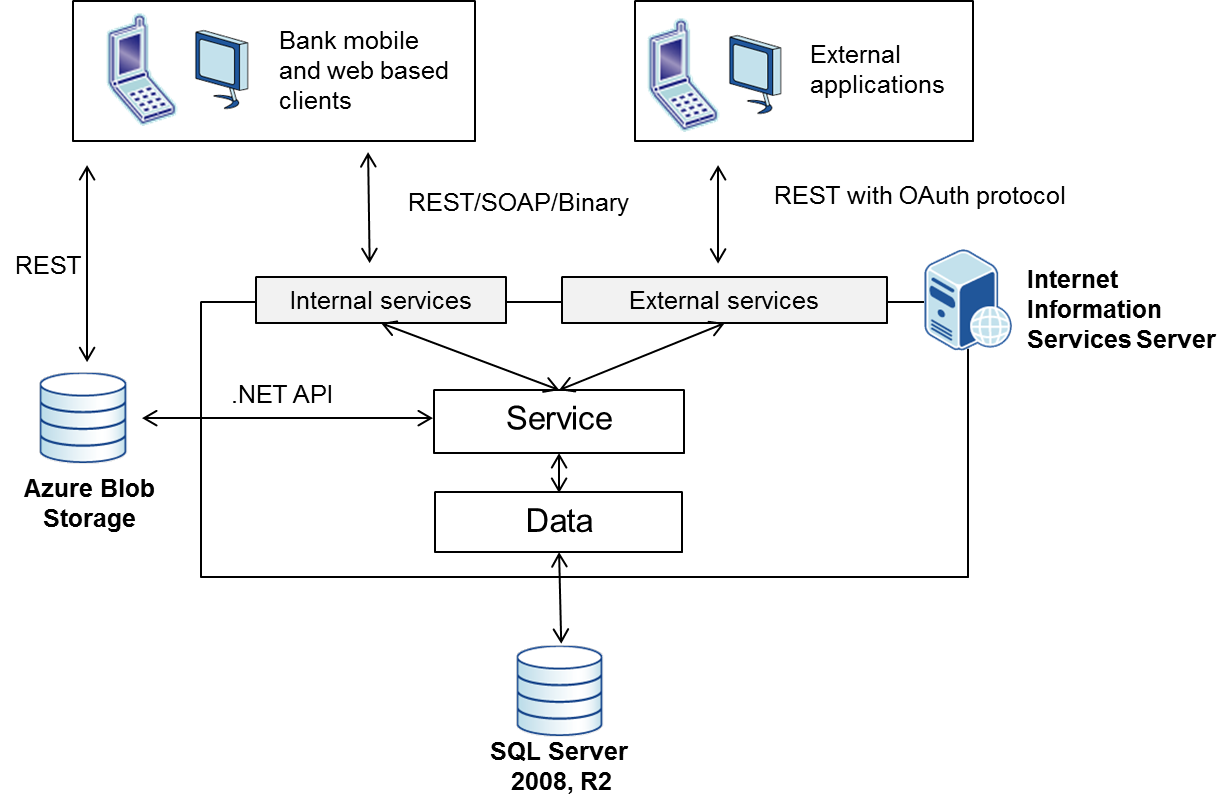
\includegraphics[width=14cm]{figures/big_picture}
\caption{High level overview of the application}
\label{fig:high_level_overview}
\end{center}
\end{figure}

The solution uses secondary non-relational (NoSQL\footnote{While the name suggest that the term refers to databases which are not using SQL language, NoSQL refers to any non-relational type of storage or database.}) storage to implement the "electronic vault" functionality. The client side applications (only the internal ones) can access the NoSQL storage directly. This has the advantage of lowering the throughput and hardware demands on the application server.

In turn the application server also communicates with the NoSQL storage in order to store directly files generated from the banking data. Figure \ref{fig:high_level_overview} summarizes the described situation.

\section{Data access layer}
The data is accessed using Object Relation Mapping (ORM)\cite{wiki:ORM}. Object relational mapping provides the layer between object model represented on the application side and entity model represented on the side of the database. NHibernate ORM framework\cite{NHib09} was chosen for this purpose. See \ref{tech:data} for comparison with other ORM frameworks. Figures \ref{fig:domain_model_1} and \ref{fig:domain_model_2} depict the domain model of the application. Figure \ref{fig:er_model} shows the entity relationship diagram of the database, based on the domain model and created by NHibernate.

Repository pattern is used to encapsulate the data persistence. Repository interfaces define the data access methods which have to be implemented and which are the only way for the business logic to interact with the database. NHibernate persistence logic is used inside the implementation of each repository. Repository pattern thus separates the data access and business layers.

Microsoft SQL Server is used as the main data storage (in the case of on-premise deployment) however the application can use any other database platform compatible with NHibernate. Since the application had to be design to run on Azure platform, the compatibility of NHibernate and Azure SQL was checked.

\section{Business layer}
\label{analysis:business_layer}
Business layer provides the core business methods of the application. As show on figure \ref{fig:appcore}, this layer makes use of the data access layer and serves the data to the communication layer, which later provides the data to several types of client applications.

Business layer is composed of several services. Each of these services concentrates on exposing methods linked with one particular type of application entities. Each service uses Dependency Injection pattern in order to resolve its dependencies specially on Repository implementations.

Dependency Injection allows decoupling of components and moves the responsibility of assembling functional components to external container object. This supports maintainability and modular structure of the project.

There are three cross-cutting concerns which are part of each business class and each business method.

\begin{description}
	\item [Logging] Technical log, which stores the information about the called method, current time and current user. These logs are not meant to be analyzed by business specialist, rather by IT experts.
	\item [Security aspects] Before the execution of each method in the business layer, the system has to determine whether the user has the right to execute the method. This depends not only on the method, but might also depend on the parameters passed to the method.
	\item [Audit trailing] Audit-trail stores the interesting information from business point of view for each significant operation. For instance for making a transfer operation containing debit account, credit account, amount and the initiator of this operation had to be stored. This data should be stored in database in order to allow future simple analysis and also for security purposes.
\end{description}

Aspect oriented programming is used in order to inject the parts of code which implement these concerns into the business methods. Spring.NET is used as Dependency Injection container and cross-cutting concerns injector. Section \ref{tech:di} discusses this choices and other Dependency Injection containers for available for the .NET platform.

\begin{figure}[h]
\begin{center}
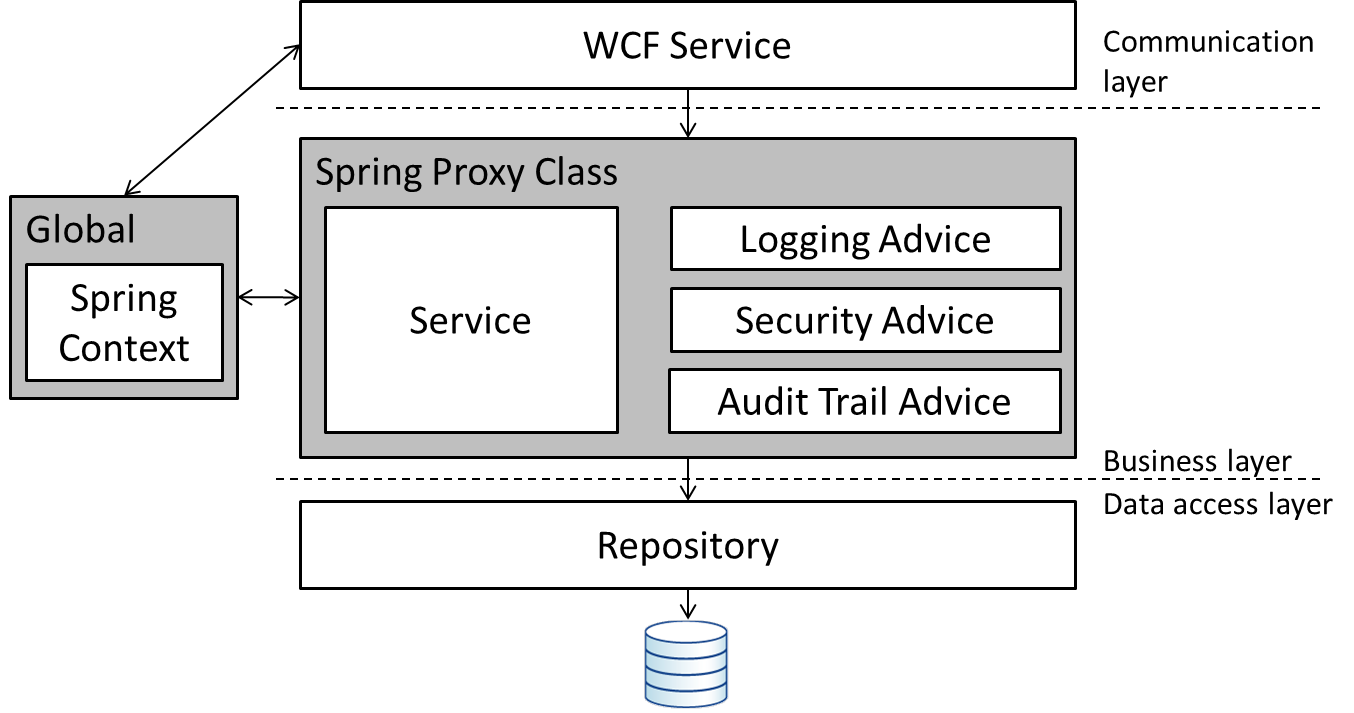
\includegraphics[width=14cm]{figures/business_layer}
\caption{The application core}
\label{fig:appcore}
\end{center}
\end{figure}


\section{Presentation layer}
Presentation layer of this application is heterogeneous. The solution is prepared to support any type of end-user client application. However in the first phase of the implementation two types of clients were implemented: web client and Windows Phone 7 client.

Both of these clients use Silverlight technology as it was required by the requester of this thesis. The standard way of designing Silverlight applications is to use Model View View-Model (MVVM) pattern. This pattern makes use of Silverlight's rich data and command binding options to separate the view from the application logic. Figure \ref{fig:preslayer} shows the usage of MVVM pattern.

The model part contains classes which reflect the server side data model. Concretely the view side model is based on data transfer objects (DTO) which are exposed by server side services.

ViewModels are represented by simple classes which hold the application logic. Each ViewModel encapsulates the logic concerned with concrete application entity. ViewModels also hold the references to the proxies of the server side services. Each ViewModel is thus responsible for getting it's own data.

View is represented by pages and controls written in XAML. XAML is a declarative language used in Windows Presentation Foundation (WPF) and Silverlight, which is used to define the user interface and define the binding between the View and the ViewModel classes.

Thanks to the MVVM pattern we can achieve almost complete separation of view and the the logic behind. As a side effect the logic of the application is isolated in ViewModel classes which are simple C\# classes and can be unit tested. Thus the whole application could run from unit tests.

\begin{figure}[h]
\begin{center}
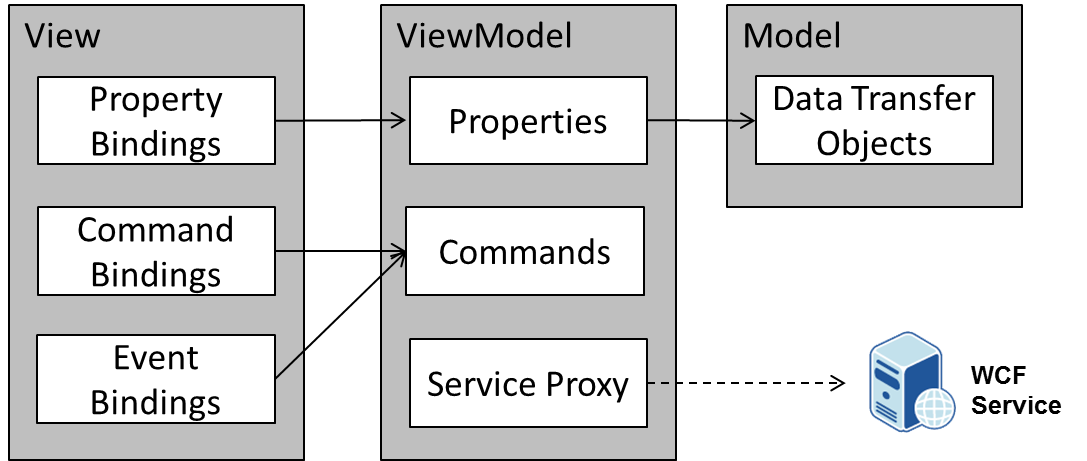
\includegraphics[width=14cm]{figures/presentation_layer}
\caption{Presentation layer}
\label{fig:preslayer}
\end{center}
\end{figure}

\section {Reusing the code between client applications}
In order to minimize the duplication of code in the web and mobile client the solution makes use of Model-View-ViewModel pattern to share the Model and ViewModel parts between both clients. However these two parts are not shared the same way.

The Model part, which contains also proxy classes to access the web service, is compiled as Portable Library project. This type of project makes the compiled assembly usable in all .NET platforms\footnote{The official version of Portable Library project was released on 15 June 2011 supporting .NET Framework, Silverlight, Windows Phone and XBOX platforms}.

The MVVM framework which was developed for this application can be with slight changes compiled for Silverlight and Windows Phone 7 platform. The same code used to define the ViewModels can be used on both platforms, however each project has to reference it's own version of MVVM framework. The solution to this situation is to link the code of the ViewModels between the Silverlight and Windows Phone 7 projects. The whole resulting structure of projects is on Figure \ref{fig:reusable_code}.

\begin{figure}[h]
\begin{center}
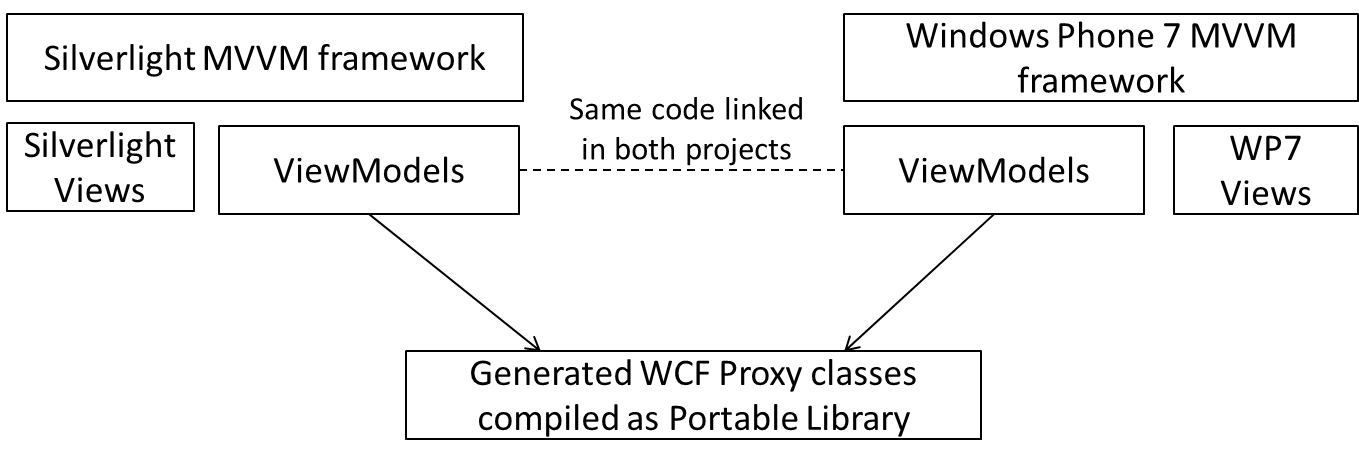
\includegraphics[width=14cm]{figures/reusable_code}
\caption{High level overview of the application}
\label{fig:reusable_code}
\end{center}
\end{figure}

\section{Communication layer}

The application server exposes separated services which provide methods and functions enabling the interaction with the banking system. Each service has a different responsibility.

Two sets of services are provided: the ones for applications developed by the bank and the external services offered for third party developers. Both sets of services are developed using Windows Communication Foundation (WCF). Section \ref{tech:wcf} discusses the main advantages of WCF.

Internal services expose the data using three different transportation formats and protocols. Binary encoding is used to transfer the data between the server and .NET based clients (Windows Phone 7, Silverlight). REST approach using JSON as transformation format is used to expose the data for other mobile clients and traditional SOAP protocol with XML as transportation format is used to enabled web services frameworks of other platforms to easily generate proxy classes (using for example Java Axis or CXF framework).

External services protected using OAuth protocol provide the data in REST-full way with JSON as transportation format.

\section{Integration of non-relational database}
\label{analysis:azureblob}
In the context of this solution a NoSQL database is used to store the client's electronic documents. This is a typical use case for which relational databases introduce higher overhead than NoSQL databases.

\subsection{Structure of Azure Blob Storage}
For this particular case Azure Blob Storage is used to perform the storage of Binary Large Objects (BLOBs). The application accesses the storage using Azure Storage account. Each Azure Storage account can have several containers. In each container several binary large objects can be stored and each blob can be composed of several blocks. Figure \ref{fig:azure_structure} shows the structure of Azure Blob Storage the way it can be used to create an electronic vault for each client.

\begin{figure}[h]
\begin{center}
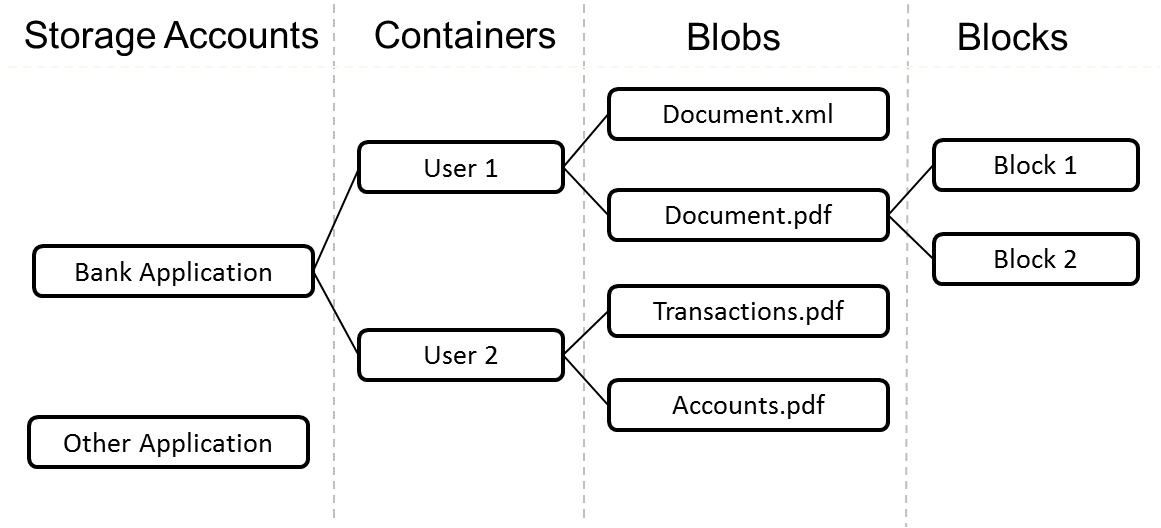
\includegraphics[width=14cm]{figures/azure_storage_structure}
\caption{Structure of Azure Blob Storage}
\label{fig:azure_structure}
\end{center}
\end{figure}

Each client possess one container, which will allow us to assign concrete rights to each container. There is no notion of folders inside of each container, but there is a special naming convention which allows overcoming of this issue.

As seen from the diagram, each file can be separated into several blocks. This is especially useful when treating large files. When file is separated into blocks, than the upload has three phases: first the list of blocks identifications is sent, than each block is uploaded separately and at last a commit is sent to the server. When some of the uploads fail, server can easily send the list of missing blocks to the client. The same applies also to download operations. This separation also allows parallel uploads by several clients.

All blobs are stored in a distributed file system in Azure Fabric\footnote{Azure Fabric is a name given to the network of interconnected computers running Windows Server 2008, which is the base of the Azure platform}. Each blob belongs to one exact partition server. Each blob has a unique key which is composed of its container name and blob name. This key is used as partitioning key, which assigns the blob to one partition server. The access to each partition server is load-balanced and all the partition servers use a common distributed file system. Because each blob has a unique partition key, than in fact the access to each blob is load-balanced, providing good throughput\footnote{In a blog post\cite{azureblob}, which dates May 2010, the Azure Storage Team stated, that the targeted throughput for a single Blob was 60Mb/s. However no other metrics were published since then.}.

\subsection{Application interfaces provided by Azure}
To interact with Azure Storage two possible application interfaces can be used.

\begin{itemize}
	\item .NET Application interface can be used from any .NET assembly running inside Azure cloud platform.
	\item HTTP REST-full Application interface can be used from any application capable of constructing and sending HTTP requests.
\end{itemize}

The access to Azure storage is protected by "storage access key" (Composed of 88 ASCII characters). Every storage account is provided with two keys (called "Primary" and "Secondary") in order to enable renewing of the access keys and keeping zero down time (both of the keys allows access to the storage at the same time).

When using the .NET API, the key is provided to the API which internally uses the key to authenticate the calls to Azure Blog Storage. When using the REST-full API, each HTTP request has to be signed by the key.

On the server side the .NET API can be used to access the storage. The server can store the key encrypted in it's configuration files. In the Silverlight client the only possibility to access the storage is to use the REST-full API. Nevertheless the key is needed to sign the requests.

\section{Security issues}
The access key cannot be given to all Silverlight clients. Silverlight application is merely a collection of files compiled into XAP package, which could be reverse engineered to obtain the key in the case of the access key hard coded inside the package. So the access has to be secured, without giving the access key to the Silverlight client application.

One option would be to build WCF service (secured by SSL) which Silverlight could ask to obtain the access key after performing authentication against the server. However this way the key would be handed to all the clients and once the attacker would infiltrate only one client machine he would also obtain non-restricted access to the whole storage account.

The second option which resolves this issue is to use Shared Access Signatures. Shared Access Signature (SAS) is a temporal authentication token which enables access to concrete blob (or whole container). This way when the client desires to access the storage, it will first contact the server and ask for Shared Access Signature. Server knowing the right information (the demanded blob or container) and being sure that the client is identified will generate the token. This token is then sent to the client using secured channel. The client can than add this token to its upload or download request which will permit him to access the demanded files. Figure \ref{fig:azure_communication} illustrates the communication between client, server and Azure Blob Storage.

\begin{figure}[h]
\begin{center}
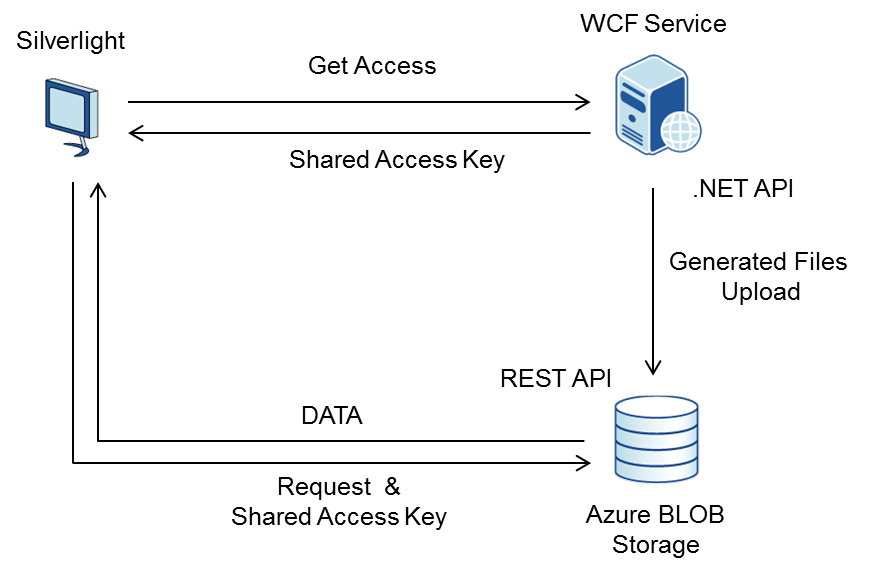
\includegraphics[width=14cm]{figures/azure_storage_calls}
\caption{Secured communication with Azure Blob Storage}
\label{fig:azure_communication}
\end{center}
\end{figure}

Even if the attacker would obtain the Shared Access Signature, the potential danger of misuse would be much lower for two reasons:

\begin{itemize}
	\item Shared Access Signature is a temporal token, valid only during limited period of time.
	\item The attacker would obtain the access just to one container or blob, not the access key which can be used to sign all requests.	
\end{itemize}

\section{Payment categorization}
\label{analysis:payment_categorization}
Automatic payment categorization uses machine learning methods to classify the transactions based on their characteristics. Each transaction has three characteristics (characteristics are sometimes referred to as features) which might be used:

\begin{itemize}
	\item  Date specifies when the transaction was made.
	\item  Amount specifies the sum of the money credited to or debited from the account. For expenses categorization only negative amounts are taken into account.
	\item  Description is a short text which describes the transactions usually originated from Core Banking System. It holds some small amount of meaningful information. For example "\textit{FACTURE CARTE DU 020811 SUPERMARCHE PARIS 06 CARTE 497}" is a short description of payment by card at the supermarket.
\end{itemize}

Out of these characteristics only the "amount" and the "description" can be used during the classification. Even though that the "amount" can hold meaningful information, it is the "description" which will have the biggest impact on the categorization.

Since the description is short text field, payment categorization is based on text categorization. Several types of classifiers can be used to perform text classification such as probabilistic classifiers, decision trees, decision rules, neural networks, example based classifiers or support vector machines \cite{Sebastiani02}.

Naive Bayes classifier does not achieve the best results (in terms of accuracy). However it achieves results comparable to other methods, is fast and relatively easy to implement comparing to more complex methods (such as decision trees, support vector machines or neural networks).\cite{XHemali09} Thus Naive Bayes classifier was chosen to implement the automatic payment categorization.

\subsection{Naive Bayes classifier}
Bayes theorem defines the probability, that an item having features $(F_1,\dots,F_N)$ has category C as\cite{wiki:naiveBayes}:

\begin{equation}
	p(C \vert F_1,\dots,F_n) = \frac{p(C) \ p(F_1,\dots,F_n\vert C)}{p(F_1,\dots,F_n)}. \,
\end{equation}

Since the denominator does not change, only the nominator is used in the probability computation.
Naive Bayes classifier assumes that all features of the classified object are unrelated, thus the conditional probability of an item having features $(F_1,\dots,F_N)$ being of class \textit{C} can be expressed as:

\begin{equation}
	\prod_{i=1}^n p(F_i \vert C)
\end{equation}

Classifier has to work with two types of features: textual (description) and continuous (amount). To enable the usage of textual features, the text has to be converted to binary vector, where each item in the vector corresponds to one word in the dictionary of all the words. If the text description contains the word, the element is set to 1, otherwise to 0.

This enables the conversion of the description of the payment to a set of binary characteristics. Each word is in fact one feature. The text "hello world" can be expressed as a vector \textit{[1,1,0,0]} using the dictionary defined at \ref{tab:word_dictionary}.

\begin{table}
\begin{center}
\begin{tabular}{|c|l|}
\hline
\textbf{index} & \textbf{word} \\
\hline
0 & hello \\
1 & world \\
2 & test \\
3 & new \\
\hline
\end{tabular}
\end{center}
\caption{Dictionary of words}
\label{tab:word_dictionary}
\end{table}

The a priori probability for each category and the conditional probability for each feature category pair have to be estimated. The a priori probability can be simply estimated as:

\begin{equation}
	P(C) = \frac{\# Items Of Category C}{\# Items}
\end{equation}

For the binary features the conditional probability of an item having class C, having feature F can be estimated as:

\begin{equation}
P(F \vert  C) = \frac{\# Items Of Category C Having Feature F}{\# Items Of Category C}	
\end{equation}

In simple terms we are estimating the probability of and item having a certain category when the description contains certain word.

The amount of the payment is continuous characteristic thus traditional Gaussian distribution can be used to estimate the conditional probability of an item having the class C.

\begin{equation}
	P(F = v \vert C) = \frac{1}{\sqrt{2\pi\sigma^2_{c,f}}}\,e^{ -\frac{(v-\mu_{c,f})^2}{2\sigma^2_{c,f}} }
\end{equation}

Before the estimation can be applied the variance ($\sigma^2_{c,f}$) and mean value ($\mu_{c,f}$) have to be computed for each feature-category pair, for all continuous features.

The transactions have to be analyzed before building the model to obtain the parameters for estimation of conditional probability. Concretely the average value and variance has to be obtained for the "amount" of the transaction and the dictionary of words has to be build for the "description" of the transactions.

\subsection{Learning process}
To learn the classifier can use two different sets:

\begin{itemize}
	\item  All categorized transactions of the concerned client.
	\item  All transactions in the system.
\end{itemize}

For most of the clients it will be safe to use all transactions in the system to learn the classifier, however there will be clients having special custom categories or categorizing some transactions in other way than majority of other clients. The wise solution would be to use all transactions only in the situation when there is not enough categorized transactions for each client.

\section{Data interfaces using OAuth protocol}
OAuth protocol is industry standard for delegation of user's rights to third party applications.\cite{OAuth11} It has been developed by cooperation of several engineers of significant internet enterprises\footnote{The group which wrote the initial draft of the protocol was composed of engineers of Google, Twitter, CitizenSpace and Ma.gnolia. The authors of current OAuth draft (version 2.22) are E.Hammer-Lahav Ed (Yahoo), D. Recordon (Facebook) and D.Hardt (Microsoft)}.

OAuth protocol is designed to solve a common situation. The user (or client) is owner of digital resources. To manage his resources the user has to authenticate himself using his credentials. In some situation we can imagine that the client would like to use third party application(s) to manage or use his resources.

Concretely in the banking scenario, the client might like to perform some analytical tasks on the data of his accounts using some third party applications such as Personal Finance Management software.

However to give the application the access to the accounts, he would be forced to share his credentials with the application. This is not desirable while, the application then would obtain full access to all of the resources. Instead using the OAuth protocol, the client can authorize the application to obtain temporal token and access the data using this token. Figure \ref{fig:oauth_workflow} shows the standard OAuth workflow applied to the situation of the bank and the client willing to access his banking data through third party application.

\begin{figure}[h]
\begin{center}
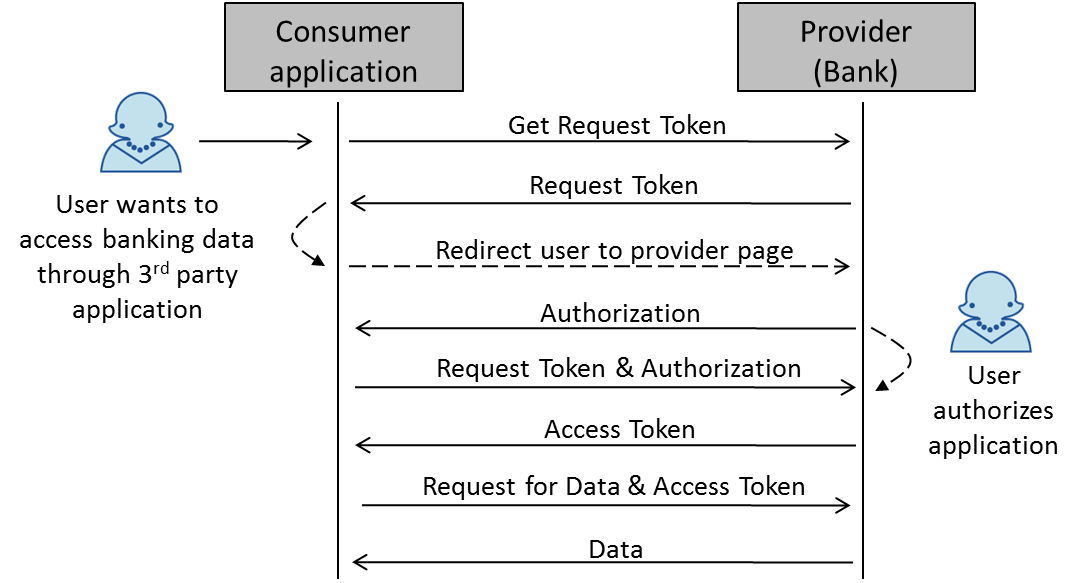
\includegraphics[width=14cm]{figures/oauth_workflow}
\caption{Workflow of the OAuth protocol}
\label{fig:oauth_workflow}
\end{center}
\end{figure}

OAuth protocol uses standard cryptographic tools such as hashing or RSA encryption to secure the HTTP requests and thus encrypting the communication. There are several existing libraries and frameworks which might be useful to facilitate the task of implementation of this protocol. Thanks to the wider possible usage most of these frameworks offer only client side OAuth implementation. There is only one library in the .NET ecosystem, which provides the infrastructure for developing the OAuth provider called DotNetOpenAuth\footnote{\href{http://www.dotnetopenauth.net/}{DotNetOpenAuth} is developed by Andrew Arnott (Microsoft), as an open source project and has been used in several large applications, such as StackOverflow or DotNetNuke}.

DotNetOpenAuth provides classes and methods which enable the developers to easily create OAuth consumer or provider and manipulate tokens. However both consumer and provider have to decide on how to handle and store the tokens and nonces\footnote{Nonce is a cryptography term describing number used only once. In OAuth protocol the nonces are used to evict replay attacks. Both nonces and tokens have to be persisted by the provider}.

The simplest architecture consists of a WCF service which returns the data and is secured by OAuth protocol. Consumer can access this services only when he obtains authorization of the actual user and owner of the resources and if he adds the negotiated token to the request. To obtain the token the consumer has to perform the OAuth "handshake" with OAuth endpoints. Figure \ref{fig:oauth_composition} shows the architecture of OAuth provider implemented using DotNetOpenAuth library.

\begin{figure}[h]
\begin{center}
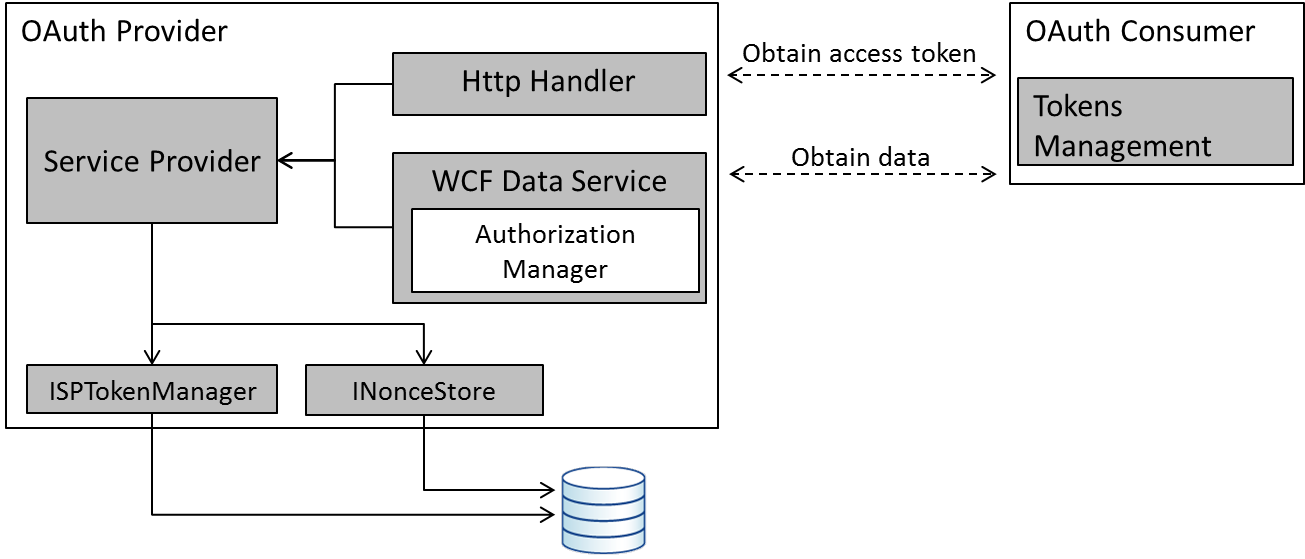
\includegraphics[width=14cm]{figures/oauth_composition}
\caption{The architecture of OAuth provider}
\label{fig:oauth_composition}
\end{center}
\end{figure}

There are two entities which perform the communication. First it is a HTTP Handler which takes care of the OAuth "handshake". The second is the actual WCF service which uses custom Authorization Manager\footnote{Authorization Manager is a WCF message interceptor, which enables definition of custom logic to decide whether the request has passed the authorization or not.} to perform the authentication. Both of these make use of the \textit{ServiceProvider} class, which is a standard part of DotNetOpenAuth library. \textit{ServiceProvider} uses implementations of \textit{IServiceProviderTokenManager} and \textit{INonceStore} also defined in DotNetOpenAuth, which take care of the persistence of nonces and tokens. It is up to the programmer to decide how to implement these interfaces.

The OAuth specification defines four endpoints. \textit{Request}, \textit{Authorize} and \textit{Access} endpoints are used to perform the handshake. The proposed architecture however proposes only one HTTP Handler to perform the handshake. That is because the handler can determine which role to take according to the incoming request. The forth endpoint is the data service.

\subsection{Persistence of OAuth entities}
Since the information about tokens, consumers and nonces have to be stored in the database, these entities have to be added to the application domain and configured to be persisted using NHibernate. 

DotNetOpenAuth already defines the infrastructure in the means of \textit{INonceStore} and \textit{IServiceProviderTokenManager} which in fact are similar to database repositories and interfaces \textit{IServiceProviderRequestToken} and \textit{IServiceProviderAccessToken} which are entities representing the tokens.

The core domain of the application is library independent and all classes are defined as poor old CLR classes. For that reason it would not be advisable to let the POCO objects in the domain implement the DotNetOpenAuth interfaces directly.

Instead of that the DotNetOpenAuth works with classes implementing the DotNetOpenAuth interfaces and these classes are wrappers for the database entities, which in fact do not implement any interfaces. This assures that the core domain of the application would not have to change if there would be different library used for the handling of OAuth protocol. Figure \ref{fig:oauth_wrapping} depicts the classes implementing DotNetOpenAuth interfaces.

\begin{figure}[h]
\begin{center}
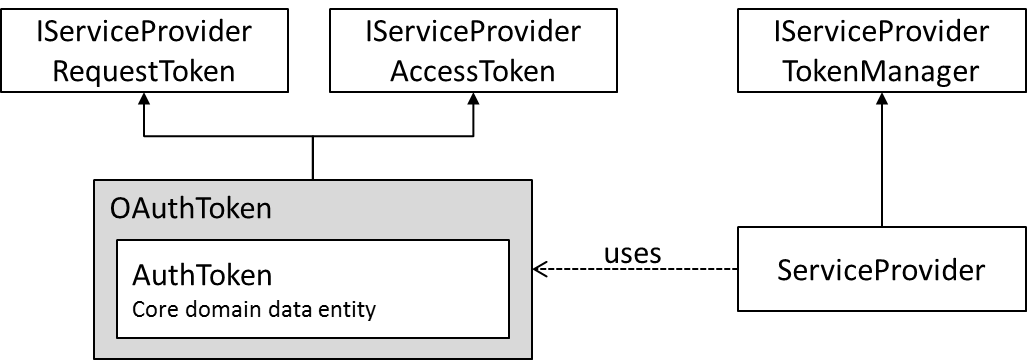
\includegraphics[width=14cm]{figures/oauth_wrapping}
\caption{Classes implementing DotNetOpenAuth interfaces}
\label{fig:oauth_wrapping}
\end{center}
\end{figure}
\chapter{Description of the implementation}

\section{Assembling the application core}
As it was described in \ref{analysis:business_layer} Spring.NET is used to assemble the business layer services. To demonstrate the steps taken to assemble the each service, a simplified version of \textit{OperationServices} class is demonstrated in this section.

First the interface for the service has to be defined (usually in the application core assembly, assembly which defines all the interfaces that build up the entire application).

\begin{verbatim} 
public interface IOperationServices
{
    IList<OperationDto> GetOperations(int accountId);
}
\end{verbatim}

The actual implementation of the service will be omitted here, but the \textit{GetOperations} method simply makes use of predefined repositories to load operations of one account and serves it as \textit{IList}.

Each of the methods has to be wrapped with advices, before the object is injected in the place where it is used. The following snippet demonstrates the audit trailing advice. This advice is used to extract and store to the database the information about the action performed, such as the method which was called and the user which initiated the method.

\begin{verbatim}
class AuditTrailAdvice : IMethodBeforeAdvice
{   
    public void Before(MethodInfo method, object[] args, object target)
    {
        var user = HttpContext.Current.User.Identity.Name;
        var className = target.GetType().Name;
        SaveToAuditTrail(DateTime.Now,method.Name,user,className);   
    }
}
\end{verbatim}
The content of \textit{Before} method is injected in each method of class to which the advice is applied. The implementations of logging and security advices are defined the same way. The implementation of security advice is more complex while it uses custom attributes and generics to discover the decoration of each method to determine whether the current user has the right to execute the method with given parameters.

Each object which is provided by the Dependency Injection container has to be declared in the Spring.NET configuration. The following snippet supposes that the \textit{OperationServices} class was defined in the \textit{Bank} assembly. Finally the created \textit{OperationServices} instance is wrapped by a proxy class to which all advices are applied (here the situation is simplified only to AuditTrailAdvice).

\begin{verbatim}
<object id="OServices" type="Bank.OperationServices,Bank"/>

<object id="Operations" type="ProxyFactoryObject">
<property name="ProxyTargetType" value="true"/>
<property name="target">
  <ref object="OServices"/>
</property>
<property name="interceptorNames">
  <list>
    <value>AuditTrailAdvice</value>
  </list>
</property>
</object>
\end{verbatim}

The business layer services are used by WCF communication services which expose the methods to clients. Because there are several WCF service and the creation of Spring application context is costly operation, the context is defined in the Global file of the web application and is created when the application is started.

For further simplification \textit{GetObject<T>(String name)} method can be defined which will look up  the demanded object in spring context and cast it to demanded interface or class.

\begin{verbatim}
public class Global:HttpApplication
{
    public static T GetObject<T>(string id)
    {
        return (T)applicationContext.GetObject(id);
    }
    protected void Application_Start(...){
    	applicationContext = ContextRegistry.GetContext();
    }
}
\end{verbatim}
The \textit{Global} class is a static class, which represents the application and is accessible from all classes within the application. By overriding \textit{Application\_Start} method the code to create the Spring.NET context is executed when the application is starting.

It is than straight forward to call the \textit{GetObject<T>} method and instantiate the business layer service needed for given WCF service.
\begin{verbatim}
public class WCFOperationService
{
    private IOperationServices oServices;
    public WCFOperationService()
    {
        oServices = Global.GetObject<OperationServices>("Operations");
    }

    public IList<OperationDto> GetOperationsByAccount(int id)
    {
        return oServices.GetOperations(id);
    }
}
\end{verbatim}

\section{Encryption of sensitive data}
The sensitive data stored in the database has to be encrypted in order to prevent the misuse, in the case where the data is in hands of unauthorized persons. There are generally three different approaches that can be taken to secure the data in database.

\begin{description}
	\item [Build-in database encryption] SQL Server since the version 2008 offers a build-in database encryption either at full database-level or at cell level.
	\item [Use of NHibernate events] NHibernate fires events such as pre-update or post-load just before the manipulation with the data stored in database. Custom logic can be written into the callbacks of these events to handle the encryption.
	\item [Implementation of user types in NHibernate] NHibernate offers the possibility to assign a user type to any property. The user type is than used to persists the property into the database. The type can define it's own process to encode and decode the value of the property before writing it into the database.
\end{description}

Out of these three choice the last one was chosen. To store sensitive data such as client's first and last name symmetric encryption is used, while to secure the password, hashing algorithm is used. Encrypting the database or columns is thus not an option when hashing is also demanded.

The pre-update and post-load events are fired every time any columns is updated or loaded, while only several columns need to be encrypted (or hashed) so additional filtering of events would have to made. The user types are thus the best choice for this use case. Defining a user type consists of implementing the \textit{IUserType} interface.

\begin{verbatim}
public class EncryptedString : IUserType
{
    public object NullSafeGet(IDataReader rs, String[] names, object ow)
    {
        object r = rs[names[0]];
        if (r == DBNull.Value)
        {
            return null;
        }
        return DesEncryptionProvider.Decrypt((String)r);
    }

    public void NullSafeSet(IDbCommand cmd, object value, int index)
    {
        object pValue = DBNull.Value;
        if (value != null)
        {
            pValue = DesEncryptionProvider.Encrypt((String)value);
        }
        var param = (IDataParameter)cmd.Parameters[index];
        param.Value = pValue;
    }
}
\end{verbatim}

The \textit{IUserType} interface contains several methods, which have to be implemented, however two of theme are cardinal: \textit{NullSafeSet} and \textit{NullSafeGet}. These methods are executed before each read or write commands is launched against the database. In the case of update or insert, the value of the property is encrypted and passed to the SQL statement. In the case of a select statement the obtained value is only decrypted.

To perform the encryption, standard classes which reside in the namespace \textit{System.Security.Cryptography} can be used. This namespace contains classes required for encryption and hashing. For encryption the DES standard is used and for hashing a 256-bit SHA is used.

\section{Service injection in the ViewModel}
The ViewModels use several services to obtain the data from the server. When Visual Studio generates the proxy of the service it creates an interface and default implementation of the interface (with a prefix \textit{Client}). The service proxy can be simple instantiated with default settings as shows the following snippet.

\begin{verbatim}
DataService dataService = new DataServiceClient();
\end{verbatim}

This assumes, that the process of the creation of the service is always the same. This assumption is not true when the ViewModel has to create different type of service depending on the current situation and environment. This situation can arise when the ViewModel is initialized in Silverlight runtime, Windows Phone 7 runtime or in unit or functional test.

To illustrate this issue, let's describe the differences of service client in Silverlight and Windows Phone 7 applications. The service proxy for Silverlight environment does not have to handle the cookies, while the cookies are already handled by the browser, while the service proxy in Windows Phone 7 has to register and take care of the cookies. Concretely all services created within the application should use the same cookie container. Thus when the service is created, it should be created with the same Cookie Container as the services created before. Figure \ref{fig:cookies_situation} visualizes the situation.

\begin{figure}[h]
\begin{center}
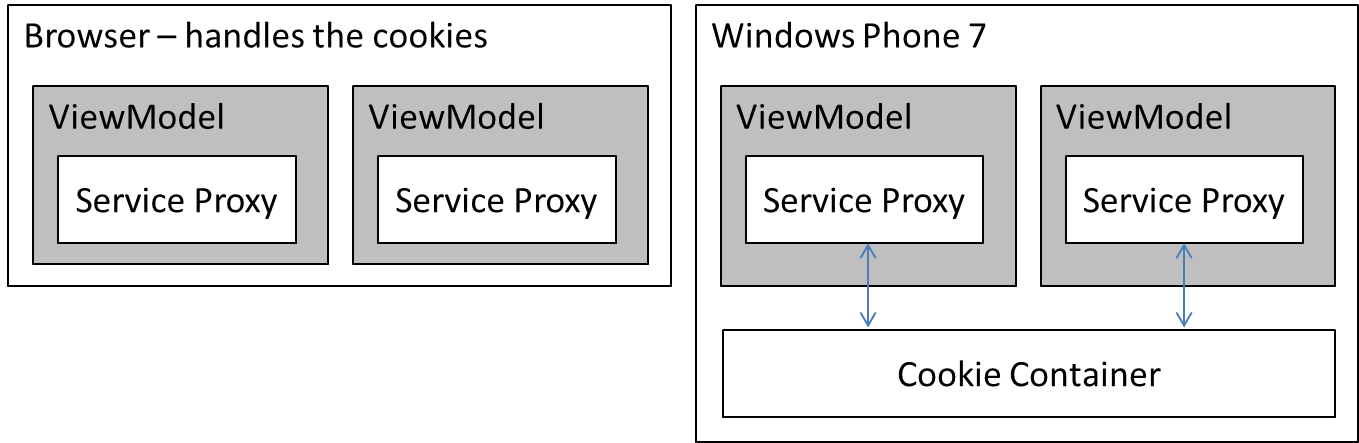
\includegraphics[width=14cm]{figures/cookies_situation}
\caption{Differences in cookies handling by Silverlight and Windows Phone 7 application}
\label{fig:cookies_situation}
\end{center}
\end{figure}

The initiation of the service in the Windows Phone 7 has to add to each service the same cookie container. This code cannot be part of the ViewModel, because than the ViewModel would not be reusable on Silverlight platform.

\begin{verbatim}
var service = new DataServiceClient();
service.CookieContainer = cookieContainer;
\end{verbatim}

For this reason the dependency injection pattern was extended to the client side. Static class \textit{ServicesFactory} contains an object implementing \textit{ICreator} interface. Different implementation of this interface can be provided depending on the situation.

\begin{verbatim}
public interface ICreator
{
    T GetObject<T>() where T : class;
}

public static class ServicesFactory
{
    public static ICreator Creator { get; set; }
    public static T GetObject<T>() where T: class {      
        return Creator.GetObject<T>();
    }
}
\end{verbatim}

The implementation of the \textit{ICreator}, which solves the problem of cookies container implements the \textit{GetObject<T>()} method using the fact that each implementation of the service has to also implement the \textit{ClientBase<T>} interface of the \textit{System.ServiceModel} namespace.

\begin{verbatim}
public Dictionary<Type, Type> services = new Dictionary<Type, Type>();

public void Register(Type iface, Type impl){
    services.Add(iface,impl);
}

public T GetObject<T>() where T : class
{
    var implem = services[typeof(T)];
    var instance = Activator.CreateInstance(implem);
    var client = instance as ClientBase<T>;
    var manager = client.InnerChannel.GetProperty<IHttpCookieContainerManager>();
    
    if (manager != null && manager.CookieContainer == null)
    {
        manager.CookieContainer = container;
    }
    
    return client as T;
}
\end{verbatim}
The implementation makes use of a dictionary of types which contains a type to be created for each interface. Before the use of the \textit{GetObject<T>()} method, this dictionary has to be filled with the interfaces and their implementations.
\begin{verbatim}
Register(typeof(DataService), typeof(DataServiceClient));
\end{verbatim}
In the ViewModel the instantiation of the WCF service is changed to the following declaration.

\begin{verbatim}
dataService = ServicesFactory.GetObject<DataService>();
\end{verbatim}
Different implementations of \textit{ICreator} can be then used for unit testing, such as an implementation which makes use of Rhino.Mock \footnote{Section \ref{tech:isolation} explains the use and choice of isolation frameworks used in this project} framework to predefine the behavior of the service.

\section{Building Model View ViewModel framework}
There exists a wide variety of MVVM frameworks, which makes the decision between them complicated. The features proposed by these frameworks are heterogeneous, but there is a set of basic functions which the MVVM framework should propose. I have identified these features and build own framework in order to achieve two aims:

\begin{itemize}
	\item Compose a framework which will contain only the features needed by the application.
	\item Compose two frameworks for Silverlight and Windows Phone 7, so that the ViewModels using these frameworks would not need any change in code and would compile for both platforms.
\end{itemize}

There are several features which can be proposed in a MVVM framework, however during the work on this thesis I have found three of them necessary.

\begin{itemize}
	\item  The possibility to create a command from lambda expressions.
	\item  The possibility to locate a ViewModel in the View which is outside of the scope defined by actual ViewModel.
	\item  The possibility to translate events into commands.
\end{itemize}

Several other features might be proposed or developed inside the MVVM framework such as tools for inter-ViewModel communication, dependency injection or background processing. However I did not found those necessary for the scope of the application.

\subsection{Creating commands from lambda expressions}
The foundation stone of MVVM pattern is the possibility of WPF or Silverlight to bind not only the properties but also the actions. Several components (such as Buttons, Panels and Lists) contain Dependency Properties\footnote{Dependency Property is a special type of a property which can be set through data binding} which expect to be bound to a property implementing \textit{ICommand} interface. This interface encapsulates an action which is executed when the command is invoked. 

This however means, that for each new command in the ViewModel a new class would have to be implemented, such as the following one:
\begin{verbatim}
public class SaveDataCommand : ICommand
{	
    public void Execute(object parameter)
    {
        DataService.SaveData(parameter as ViewModel);
    }
    
    public void CanExecute(object parameter)
    {
        parameter != null;
    }
}
\end{verbatim}

This would cause a lot of boiler plate code for every new command. Since it is only the content of \textit{Execute} and \textit{CanExecute} methods which changes for each command, generic implementation of the \textit{ICommand} interface can be invented.

\begin{verbatim}
public class GenericCommand<T> : ICommand
{
    private readonly Action<T> execute;
    private readonly Predicate<T> canExecute;
    
    public GenericCommand(Action<T> ex, Predicate<T> canEx = null){
       execute = ex;
       canExecute = caEx;
    }
    public bool CanExecute(object parameter)
    {
        return canExecute == null ? true : canExecute((T)parameter);
    }
    
    public void Execute(object parameter)
    {
        execute((T)parameter);
    }
}
\end{verbatim}
This generic class can greatly simplify the creation of new commands. In the ViewModel a new command can be defined using lambda expressions in one line of code.

\begin{verbatim}
public ICommand SaveDataCommand
{
    get { return new GenericCommand<UserData>(
       (x) => DataService.SaveData(x),
       (x) => x.Name != null);
    }
}
\end{verbatim}
This assignment defines the action which should be execute as \textit{DataService.SaveData(param)} and supposing that the \textit{UserData} object contains property \textit{Name} the action will get executed only if the \textit{Name} is not null.

\subsection{Binding to events}
Not all visual components expose Dependency Properties which could be bound to \textit{ICommand} interface. Several graphical components expose only events. Therefor there is a need for simple way to create a command from an event. The solution here is to implement a class based on \textit{TriggerAction<T>}. This class can be attached to an arbitrary event of a graphical user element of generic type T. By overriding the \textit{Invoke} the action can be defined which should be executed when event is fired.

\begin{verbatim}
public class EventToCommand : TriggerAction<FrameworkElement>
{
    //Command and Parameter have to be backed up by Dependency Properties
    //in order to enable binding
    public bool BindParameters {get;set;}
    public ICommand Command {get;set;}
    public object Parameter {get;set;}
    
    protected override void Invoke(object parameter)
    {
       if (parameter != null && BindParameters)
       {
          Parameter = parameter;
       }
       
       if (Command != null)
       {
          Command.Execute(CommandParameter);
       }
    }
}
\end{verbatim}
To use this class the \textit{Command} property has to be bound to a value in ViewModel. The Boolean value \textit{BindParameters} specifies if the parameter of the event should be passed directly as the parameter to the command. Any other object can be passed as the parameter by binding the \textit{Parameter} property.

The following snippet demonstrates the binding of "drop" event of a grid component.

\begin{verbatim}
<Grid>
	<i:Interaction.Triggers>
	    <i:EventTrigger EventName="Drop">
	        <mvvm:EventToCommand Command="{Binding Path=DropCommand}" ... />
	    </i:EventTrigger>
	</i:Interaction.Triggers>
</Grid>
\end{verbatim}

\subsection{Locating ViewModels}
When the \textit{DataContext} property of a particular View or User Control is set to certain ViewModel, then it is straightforward to bind TextBoxes, Labels or collections of this View to the values of selected ViewModel. The ViewModel "backs up" the View.

It turns complicated when there is a need to bind to values external to this ViewModel. Typical example of this situation is illustrated on figure \ref{fig:mvvm_locator} where a collection of items is show in a list. Each item contains a "remove" button which has to be bound to command defined in the parent ViewModel. Because each item in the list is bound to it's own ViewModel, the binding has to leave the \textit{DataContext} and bind to external (in this case parent) ViewModel.

\begin{figure}[h]
\begin{center}
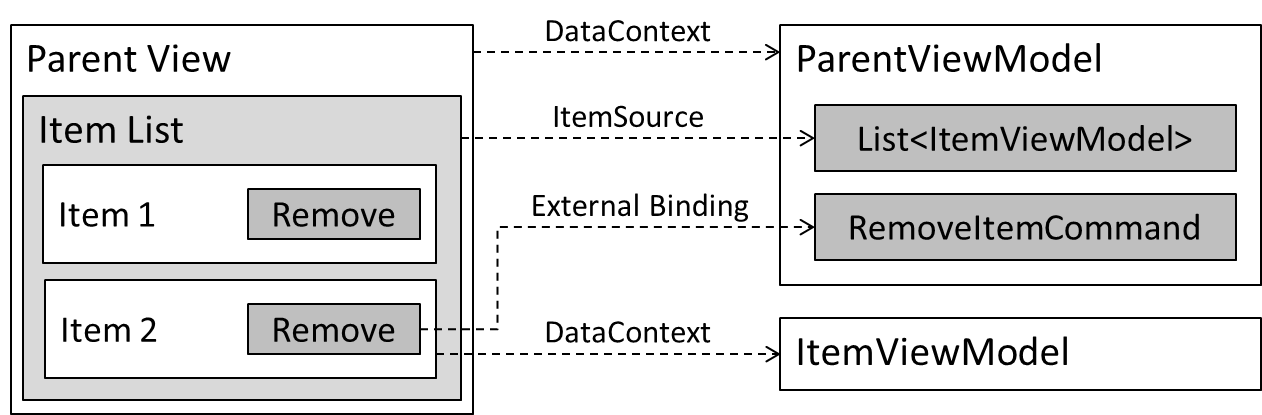
\includegraphics[width=14cm]{figures/mvvm_locator}
\caption{Binding to out of the scope ViewModel}
\label{fig:mvvm_locator}
\end{center}
\end{figure}

The solution to this issue is to create ViewModel locator class which is able to locate the ViewModel outside of the current \textit{DataContext} of current View and provide the properties of this ViewModel to the current View. One of the ways to implement this class is to create a component which can be placed to the XAML definition of the View and which will traverse the tree of graphic components and check the \textit{DataContext} of each component until it finds the demanded ViewModel.

\begin{verbatim}
public static object WalkUpTreeTillVM(this FrameworkElement obj, string vmName)
{
    var parent = obj;
    while (parent != null)
    {
        var context = parent.DataContext;

        if (context != null && context.GetType().Name == vmName)
        {
            return context;
        }

        parent = VisualTreeHelper.GetParent(parent) as FrameworkElement;
    }
    return null;
}
\end{verbatim}
In order to be able to use the result of the above stated method, \textit{ViewModelLocator} class is defined, which inherits from \textit{FrameworkElement} thus can be inserted directly into the XAML definition of the View.

\begin{verbatim}
public class ViewModelLocator : FrameworkElement
{
	public String ViewModelName {get;set;}
	
	//the Data property has to be backed up by Dependency Property to be bindable
	public object Data {get;set;}
	public DependencyProperty _data;

    protected void Loaded(object sender, RoutedEventArgs e)
    {
        if(ViewModelName != null)
        {
            //create binding between the component found by the traversing 
            //of the UI tree and the Data property
            Binding binding = new Binding();
            binding.Source = this.WalkUpTreeTillVM(ViewModelName);
            SetBinding(_data, binding);   
        }
    }
}
\end{verbatim}
Later this \textit{ViewModelLocator} can be used in the View, where the component which needs the data of particular ViewModel will bind to the exposed \textit{Data} property of this element.
\begin{verbatim}
<mvvm:ViewModelLocator x:Name="Parent" ViewModelName="ParentViewModel"/>

<ListBox ItemsSource="Items">
  <ListBox.ItemTemplate>
    <TextBlock Text={Binding Title}/>
    <!-- Command's binding is directed to the "ParentViewModel" -->
    <Button Command="{Binding Data.RemoveCommand,ElementName=Parent}"/>
  </ListBox.ItemTemplate>
</ListBox>
\end{verbatim}

\section {Implementation of Naive Bayes classifier}
Naive Bayes classifier has been implemented as new module to \textit{\href{machine.codeplex.com}{machine.codeplex.com}} library. The theoretical background is described in the section \ref{analysis:payment_categorization}. This section explains the implementation details.

The library \textit{machine.codeplex.com} contains two interfaces which define template for each new classifier: \textit{IModel} and \textit{IPredict}. The \textit{IModel} interface defines \textit{Generate} method which takes in the training data and creates an instance of \textit{IPredict}. The purpose of the model is the creation of the predictor, which in fact is ready to use classifier. \textit{IPredict} interface defines method \textit{T Predict(T item)} which assigns the category to given item.

Some additional methods are defined on both of these interface (such as serialization of the predictor to XML), but these methods are not important for banking application, therefor are not discussed.

The \textit{NaivaBayesModel} class converts all of the data in the learning set into matrix representation. Some of the internal structures of the \textit{machine.codeplex.com} library were changed to enable work with non-integer type categories.\footnote{Each transaction contains a property \textit{Tag} of the same type. Initially the \textit{machine.codeplex.com} library was not prepared to work with complex objects. Instead of that, categories of items had to be defined only using integer or double type values} In the process of converting to the matrix, a dictionary of tags is made and than only the integer index is used to reference each tag.

\subsection{Construction of the predictor}
The predictor needs four structures to hold important data in order to classify the item according to textual or continuous characteristics. These structures are one or two dimensional arrays. Each category or feature has assigned index (during the pre-processing) which enables the look-up in these arrays.

\begin{verbatim}
//Posteriori probability for each feature-category pair
//(where feature is binary property)
public double[ ][ ] Posteriori;

//A priori probability for each category
public double[ ] Apriori;

//Average value for each category-feature (where feature is continuous property)
public double[ ][ ] CategoryFeatureAvg;

//Variance for each category-feature (where feature is continuous property)
public double[ ][ ] CategoryFeatureVariance;
\end{verbatim}
The computation of a priori probability is the same for both type of features. 
\begin{verbatim}
Apriori[i] = CategoryCount[i] / TotalCount;
\end{verbatim}

The computation of a posteriori probability is done only for binary characteristics (containing the textual characteristics converted into binary characteristics).
For the binary features, the value at position [i,j] will be computed as follows.
\begin{verbatim}
Posteriori[i][j] = CategoryFeatureCount[j][i] / CategoryCount[i];
\end{verbatim}
Applied to the textual characteristics, this formula simply says that the probability of a text having category C with index (i) and containing word W (with index j) is the count of the items having the word W and category C divided by the total number of items having the category C.

For the continuous features, the posterioiri probability is estimated using the Gaussian distribution, using the average and variance values. The data arrays which contains average values and variances has to be filled before by the analysis of items in learning set. 

\begin{verbatim}
Normal(CategoryFeatureAvg[i][j],CategoryFeatureVariance[i][j],value)
\end{verbatim}

\subsection{Categorization process}
Once the arrays containing the a priori probability for each category and a conditional probability for each category-feature combination are prepared, the process of classification of an item consists of computing the probability of the item having the category for each category. The category with highest probability value will be selected.

To process the computation for one item and one category the classification has to loop over all features and multiply the probabilities.

\begin{verbatim}

foreach (var category in Categories)
{
  for (var feature in Features)
  {
      if(feature.IsContinuous){
      {
          var estimation = Normal( 
          			  CategoryFeatureAvg[category][j],
          			  CategoryFeatureVariance[category][j],
          			  value);
      }

      if (feature.Type.IsBinary))
      {
          var estimation = Posteriori[category][j];
      }
      probability = probability * estimation;
  }

  if (probability > maxProbability)
  {
      maxProbability = probability;
      maxCategory = category;
  }
}
item.SetValue(maxCategory);

\end{verbatim}
The process is composed of two loops, the type of each feature is determined (continuous or binary) and appropriated method is selected to get the value of the conditional probability. The classifier remembers the category which obtained the highest probability and the last statement categorizes the item.

\section {Using face recognition for easier authentication}
Face recognition is complicated machine learning task. The process of face recognition has two phases:

\begin{description}
	\item [Face detection] Face detection is the process of detecting the pixels in the image which represent the face. 
	\item [Face recognition] The actual task of recognizing the face by analyzing the part of the image identified during the face detection phase.
\end{description}

Face recognition brings in several problems which are completely unique to this domain and which make it one of the most challenging in the group of machine learning problems.

\begin{description}
	\item [Illumination problem] Due to the reflexivity of human skin, even a slight change in the illumination of the image can widely affect the results.
	\item [Pose changes] Any rotation of the head of a person will affect the performance.
	\item [Time delay] Due to the aging of the human individuals, the database has to be regularly updated.
\end{description}

\subsection{Eigenface-based face recognition}
There are several methods and algorithms which can be used to perform face recognition. Section \ref{tech:face_recognition} discusses the different methods. Eigenface algorithm was chosen because of the availability of several open source implementations and because of it's relative simplicity. Section \ref{tech:eigenface} describes the details of the algorithm.
The algorithm is based on Principal Component Analysis (PCA) and as such, follows the pattern applied by other statistical methods:

\begin{itemize}
	\item Compute the distance between the captured image and each of the images in the database.
	\item Select the example from the database, which is closest to the processed image (the one with the smallest distance to captured image). If the distance is not too big – label the image as concrete person. 	
\end{itemize}

The eigenfaces algorithm therefor has to define how to compute the distance between two images. To overcome this issue the PCA algorithm creates a set of principal components, which are called eigenfaces. Eigenfaces are images, that represent the main differences between all the images in the database.

The recognizer first finds an average face by computing the average for each pixel in the image. Each eigenface represents the differences from the average face. First eigenface represents the most significant differences between all images and the average image and the last one the least significant differences.

Figure \ref{fig:avarage_face} visualizes the average image created by analyzing the faces of 10 consultants working at OCTO Technology, having 5 images of each consultant. Figure \ref{fig:eigenfaces} shows the first five eigenfaces of the same dataset.

\begin{figure}[h]
\begin{center}
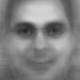
\includegraphics[width=3cm]{figures/avg}
\caption{Average face}
\label{fig:avarage_face}
\end{center}
\end{figure}

\begin{figure}[h]
\begin{center}
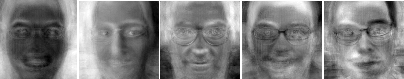
\includegraphics[width=10cm]{figures/eigenfaces}
\caption{First five eigenfaces created by analyzing images of 10 consultants working at OCTO Technology}
\label{fig:eigenfaces}
\end{center}
\end{figure}

After the creation of the eigenfaces, each image can be represented as a composition of these faces. Each image can be thus represented as a vector, where the elements of the vector are the coefficients given to each eigenface.

The distance between two images can be computed as the distance between two points in N-dimensional space, where N is the number of eigenfaces. For computing the distance, the Euclidean distance formula is used.

\subsection{Open Source libraries for Eigenfaces algorithm}
Eigenfaces based algorithm has already been developed in several languages and is available as part of existing image processing and machine learning libraries. To use eigenfaces in C\# EmguCV library can be used. EmguCV is a .NET wrapper for OpenCV library, written in C++ by Intel and published as open-source.\footnote{OpenCV library is released under BSD license and is free for academic and commercial use. It has been written in C++, with C and Python interfaces. EmguCV is written in C\# and uses the ability of .NET code to call methods from unmanaged assemblies.}

Using EmguCV means that any function inside OpenCV library can be called without the need of using constructs such as \textit{DLLImport} directive and without the need of knowing the exact structure of the OpenCV library.

The fact that EmguCV uses unmanaged DLL libraries, can pose problems for application interoperability. When compiled, .NET assemblies and programs are designed to run on every processor. If the the solution uses unmanaged libraries it is usually safe to include 32-bit assemblies, to assure the compatibility of the program on 32-bit machine.

However Azure cloud platform runs on 64-bit machines and furthermore it is not possible to load 32-bit library on this platform. Thus 64-bit versions of all external DLL libraries have to be used.

Including 64-bit assemblies can rise another issues also while developing and testing the software. The web server integrated in Visual Studio which is usually used for debugging (called Cassini) supports only 32-bit applications. Thus a local IIS server has to be created for debugging and testing.

\subsection{Process of face recognition}
The majority of the face recognition process is executed on the server side. Figure \ref{fig:face_recognition} depicts the phases in the training and face recognition processes.

\begin{figure}[h]
\begin{center}
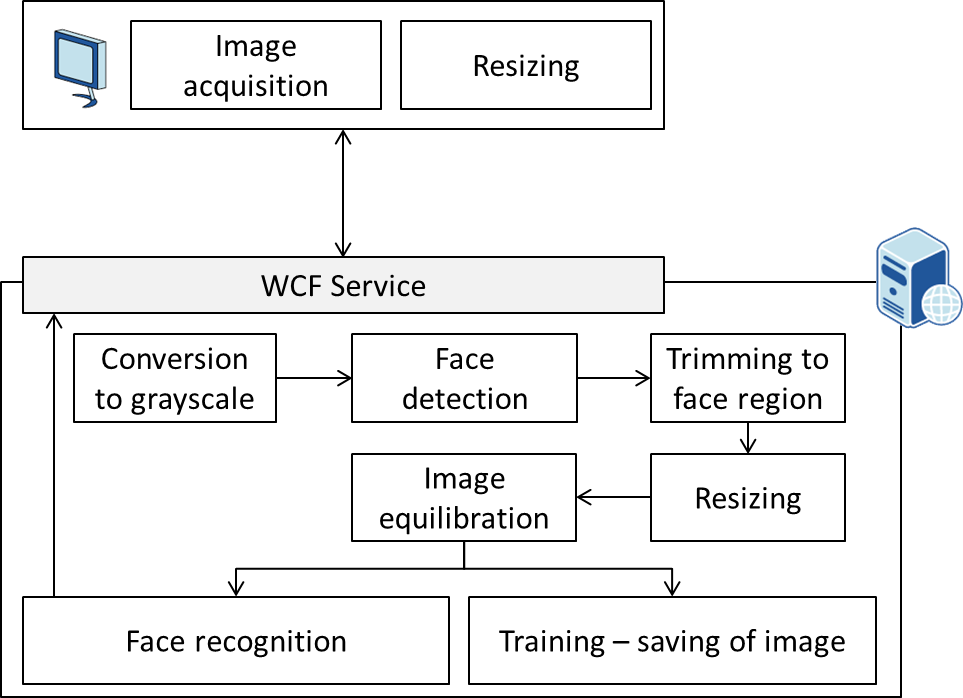
\includegraphics[width=14cm]{figures/face_recognition}
\caption{The process of face recognition}
\label{fig:face_recognition}
\end{center}
\end{figure}

\subsection{Capturing the image}
Since the version 4 Silverlight gives us the possibility to use the camera to capture images or videos using the \textit{CaptureSource} class. The following snippet shows how to access and start the camera.
\begin{verbatim}
var source = new CaptureSource();
source.VideoCaptureDevice = 
CaptureDeviceConfiguration.GetDefaultVideoCaptureDevice();
source.CaptureImageCompleted += 
new EventHandler<Args>(captureCompleted);

if (captureSource.State != CaptureState.Started)
{   
    if (CaptureDeviceConfiguration.RequestDeviceAccess())
        captureSource.Start();
}	
\end{verbatim}
To visualize the content of \textit{CaptureSource} the \textit{VideoBrush} can be used and applied to any graphical component (such as Rectangle or Ellipse).

\begin{verbatim}
var vidBrush = new VideoBrush();
vidBrush.Stretch = Stretch.Uniform;
vidBrush.SetSource(captureSource);
Rectangle.Fill = vidBrush;	
\end{verbatim}

Silverlight is asynchronous environment, where the user interface thread (UI thread) cannot be used by blocking operations. For that reason the developer has to set the callback for the \textit{CaptureImageCompleted} event. The following code is executed within the callback.

\begin{verbatim}
private void captureCompleted(Object sender, Args e)
{
    var image = e.Result;
    switch(appMode)
    {
        case AppMode.Recognition:
            client.RecognizeAsync(image.Pixels);
            break;
        case AppMode.Training:
            client.TrainFaceAsync(image.Pixels, label);
    }
}
\end{verbatim}

As a result of the capture, \textit{WritableBitmap} object is obtained, which has a \textit{Pixels} property of type \textit{int[]}. This property holds all the pixels of the image in one dimensional array created by aligning all the rows of the image to one array. Each pixel is represented as \textit{Integer}. Each color is thus represented using 32-bits.

This array has to be sent to the server. When the application is in training mode, also the label of the image is sent. If the application is in recognition mode, only the image is sent and the label of the image should be received.

\subsection{Server side recognition process}
Face recognition has two phases: face detection and face recognition. EmguCV can be used for both tasks. 

The first step which has to be taken is the detection of the face and clipping of the image. EmguCV uses \textit{Image<color type,depth>} structure for treating images, so the array of pixels has to be converted to this representation. Later the application uses the \textit{HaarCascade} class to perform the face detection. Section \ref{tech:haarcascade} contains additional information about Haar Cascade face detection.

\begin{verbatim}
var inBitmap = ConvertToBitmap(pixels, iSize);
var grayframe = new Image<Gray, byte>(inBitmap);
var haar = new HaarCascade(getHaarCascade());

var faces = haar.Detect(grayframe,
						  1.2,
						  3,
						  HAAR_DETECTION_TYPE.DO_CANNY_PRUNING,
						  new Size(30,30));
	
if (faces.Count() != 1)
    return null;

var face = faces[0];
var image = grayframe.Copy(face.rect);
\end{verbatim}

The image is converted to gray-scaled image where each pixel has 8 bits. Once the face is detected (and if there was only one face), the rectangle encapsulating the face is copied to a new image structure. Before passing the image to the recognition, we can reduce the noise created by different illumination situations by equalizing the image.

Histogram equalization is a technique to improve the contrast and adjust the brightness of the image. EmguCV gives us the possibility to call the equalize function which resides in OpenCV. Figure \ref{fig:image_equalization} visualizes the changes done by image equalization.

\begin{figure}[h]
\begin{center}
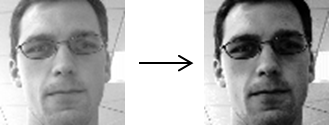
\includegraphics[width=8cm]{figures/equalization}
\caption{Image equalization}
\label{fig:image_equalization}
\end{center}
\end{figure}

For recognition task EmguCV contains \textit{EigenObjectRecognizer} class, which needs several arguments to be created:
\begin{description}
	\item [Images and labels] Array of images and corresponding array of labels.
	\item [Eigen Distance Threshold] Eigenfaces algorithm measures the distance between images. This thresholds defines the maximal distance needed to classify the image as concrete person. Big values such as 5000 will make the classifier to return the closest match, even if the probability that the person has been recognized is quite small. Values around 500 assures reasonable results.
	\item [MCvTermCriteria] \textit{McvTermCriteria} is a class which represents OpenCV structure for terminating iterative algorithms. It is composed of two numbers the first being the number of iterations and the second one is demanded accuracy. For some algorithm it makes sense to iterate until the accuracy is not bellow certain threshold. For eigenfaces algorithm it is the number of iterations which is important and it will impact the number of eigenfaces created.
\end{description}

The actual face recognition uses the method defined above to detect and trim the face. The resulting image is than passed to the recognizer. And the found label is passed through WCF service to the client application.

\begin{verbatim}
var termCrit = new MCvTermCriteria(40, accuracy);
var recognizer = 
	new EigenObjectRecognizer(trainedImages,labels,
             		eigenDistanceThreshold,ref termCrit);
             		
var imgFace = DetectAndTrimFace(pixels, size);
var label = recognizer.Recognize(imgFace);
\end{verbatim}

The face-detection phase is quite instantaneous. OpenCV already offers a set of HaarCascade features. The creation of these features is much more time consuming, than their usage.

If the database of faces does not change, the recognizer can be created only once and than can be shared every-time there is a request for recognition. This of course is not possible when the image database changes. In that case the recognizer has to be  recreated. There is no possibility to add new image to existing recognizer.

The bottleneck of this approach is still the network over which the image has to be passed from the client to the server. To minimize the data which has to be transferred, alternative approach could be used with face detection on the client side, which would lower the amount of pixels to be transferred to the server side. \footnote{There is an open-source project \href{facelight.codeplex.com}{facelight.codeplex.com} written for Silverlight which uses search for skin color regions and might be used to perform the face recognition on the client side.}.

\section {Implementation of Electronic vault}
Azure Blob Storage proposes two types of application interfaces. 

\begin{itemize}
	\item .NET Application interface
	\item HTTP REST Application interface
\end{itemize}

.NET API is a set of classes which can be used on the server side to access the storage. The following snippet shows, the process of uploading the file to Azure Blob Storage using only the server side interface.

\begin{verbatim}
var account = CloudStorageAccount.FromConfigurationSetting("connStr");
var client = account.CreateCloudBlobClient();

var container = client.GetContainerReference("container");
container.CreateIfNotExist();
var blob = container.GetBlobReference("fileName");
blob.UploadByteArray(data);
\end{verbatim}

The connection string which is used to connect to the storage contains the applications access key. This API runs only within the Azure environment. This means that application which would like to make this type of server side calls has to be deployed to the Azure platform.

REST API is completely platform independent and uses HTTP as its transport protocol to execute actions, upload and download data from the storage. The creation of the HTTP request depends on the platform of the client. In C\# we can use the following code:

\begin{verbatim}
public void UploadFile(Uri url){
  var request = (HttpWebRequest)ClientHttp.Create(url);
  request.Method = "PUT";
  request.Headers["x-ms-meta-comment"] = "my comment";
  request.Headers["x-ms-meta-author"] = "current user";
  request.BeginGetRequestStream(WriteData, webRequest);
}

private void WriteData(IAsyncResult result)
{
  var request = (HttpWebRequest)result.AsyncState;
  var stream = webRequest.EndGetRequestStream(result);       
  stream.BeginGetResponse(UploadFinish, webRequest);
}

private void UploadFinished(IAsyncResult result)
{
  if(result.IsCompleted){
    //Check the response
  }
}
\end{verbatim}

Note that the metadata of the file (comments, author) are added as headers to the HTTP Request.

In the proposed implementation it is advantageous to use both application interfaces. To give the Silverlight client direct access to the storage the REST API is used. This will also avoid passing of all the data through WCF Services and take significant data load of the servers. In case of generation of documents (such as transaction overviews), the documents will be generated and inserted to the vault using the server side API.

Is it has been explained in \ref{analysis:azureblob} Shared Access Signature mechanism is used to secure client side calls.
The generation of Shared Access Signature on the server side is simplified by the .NET API, which provides required methods. The following snippet illustrates the generation of Shared Access Signature, which will give the user read rights for the next 10 minutes.

\begin{verbatim}
var container = client.GetContainerReference("container1");
var permissions = new BlobContainerPermissions();
permissions.PublicAccess = BlobContainerPublicAccessType.Off;
container.SetPermissions(permissions);

var expDate = DateTime.UtcNow + TimeSpan.FromMinutes(10);
var sas = container.GetSharedAccessSignature(new SharedAccessPolicy()
{
   Permissions = SharedAccessPermissions.Read
});
\end{verbatim}

\subsection{Comparison with regular database}
The electronic vault could be also implemented using a SQL Server or Azure SQL (equivalent Cloud offer to SQL Server), by storing the files in the relational database. Here is a list of advantages which Azure Blob Storage has over relational database.

\begin{itemize}
	\item Blob Storage offers build-in support for the metadata for each file.
	\item Blob Storage has the ability of separating the files into blocks and thus provides better support for treatment of large files.
	\item The architecture of Blob Storage allows the access to each blob to be load-balanced and thus provides high access speed. However due to the dependence on network connection this is difficult to compare with SQL Server on premise or Azure SQL and no metrics have been published by Microsoft.
\end{itemize}
\chapter{Testability of the solution}
This chapter describes the set of tests which are used to prove the quality of the code. The solution was designed for testability. In total there are five types of tests to stress the quality and correctness of the code.

\begin{itemize}
	\item  Standard unit tests to cover the business and data access layer.
	\item  Parametrized unit tests to increase the coverage of the business layer.
	\item  Unit test for ViewModels in the presentation layer.
	\item  Functional tests to test the whole application.
	\item  Load tests for performance analysis.
\end{itemize}

\section{Standard unit tests}
Standard unit tests were defined to verify the correctness of Data Access and Business layers. To isolate the tested code from the rest of the application Rhino Mock framework is used. See \ref{tech:unit} for the justification of this selection. In order to test the database persistence and the whole Data Access layer SQLite\footnote{\href{http://www.sqlite.org/about.html}{SQLite} is a embedded relational database framework, which runs without any separated server-side process. The data is stored in regular disk files.} database is used.

\section{Parametrized unit tests}
To exercise each path in the tested unit or method, several unit tests have to be written manually. For each of these tests the data has to be prepared and also the mocks prepared for each interacting component. This results in lot of repetitive code. This situation can be illustrated by the following code snippets. Assume that we have one method to test:

\begin{verbatim}
void Transfer(int creditId, int debitId, int amount) {}
\end{verbatim}

The above specified method uses the ID's of credit and debit accounts and adequate repository class to find these accounts. If both accounts were found, the method checks whether the transfer can be done. Some accounts may authorize the overdraft some not. This results in a set of tests:
\begin{itemize}
\item Credit and debit accounts are the same.
\item Credit account was not found.
\item Debit account was not found.
\item Amount is bigger than debit account balance and overdraft is not authorized. 
\item Amount is bigger than debit account balance and overdraft is authorized.
\item All parameters are correct
\end{itemize}
At least the 5 above mentioned tests should validate the method and make sure, that appropriate exception will be thrown when preconditions are not kept or other issues arise.

Parametrized unit tests are designed to simplify this situation. The signature of parametrized testing method will be usually the same as the signature of tested method. The parameters which are given to this method will vary. Parametrized testing framework can be used to automatically divine the parameters to exercise all paths in the method. In this solution Pex framework was used, which allows the creation of following parametrized unit test:

\begin{verbatim}
//a field which holds testing data
accounts = GetTestingAccountsData();

[PexMethod]
public void MakeTransfer(int debitId, int creditId, decimal amount)
{
    var repository = new SIRepository();
    
    //the repository will look up the accoun in testing data
    repository.GetObject<Account>((x) => 
    			accounts.SingleOrDefault(a => a.Id == (int)x));
	
    var operationServices = new OperationServices(repository);
    
    operationServices.Transfer(debitId, creditId, amount);
}
\end{verbatim}

Parametrized testing method initializes the target (\textit{OperationServices} class) and than passes the parameters to the tested method. A repository has to be given to the services class, in order to enable the service to find the accounts in the database according to the id's. In the code above the repository is mocked using \textit{SIRepository} mole class. This class is created using the Moles framework \ref{tech:moles}.

A delegates is passed to the \textit{GetObject} method which states that every time this method is called to look up an Account object in the repository, it will look the object up in a predefined field \textit{accounts} which can be any \textit{IEnumerable} object holding testing data.

Pex analyzes all the branches in tested method and initializes the parameters to cover each of the branches. Each of the set of parameters generated by Pex can than be stored as a new unit test. Instead of writing five unit testing methods, only one has to be written, assuming that Pex is able to generate the parameters. Section \ref{tech:parametrized_testing} discusses the technical details of parametrized unit testing using Pex framework.

\section{Unit testing the ViewModels}
One of the advantages of MVVM pattern is the ability to test the logic in the user interface. ViewModels are standard C\# classes however they reside in Silverlight assembly. Silverlight assemblies cannot be loaded into the Visual Studio test host environment. As the solution to this issue a specialized testing host environment is a part of Silverlight Toolkit. While using the Silverlight Toolkit, the tests can be written as standard unit tests. The only difference is that the tests are executed in the test host inside a web browser as a Silverlight XAP package.

The perimeter of the ViewModel testing is quite small, while all of the network calls have to be mocked and requires lot of boiler plate code. Most of the code of the ViewModels should also be tested by acceptance tests, therefor it is question to which extend the ViewModels should be tested two times (by unit as well as acceptance tests).

\section{Acceptance tests}
Acceptance test is a test which is conducted to determine if the requirements on the software are met\cite{wiki:acceptance}. In the context of software engineering project, it is useful when the tests are written by stakeholders with knowledge of the functional domain. The tests are usually written in business domain language. Acceptance tests are a sub-group of functional tests. Functional tests are black-box tests which are executed to determine the good functionality of the software. Acceptance tests are functional tests which also define concrete requirements based on the specification or contract.

Several acceptance testing frameworks exists which can be used to define the test in "easily understandable" language and executed automatically.

To define the tests on this solution FitNesse\footnote{FitNesse is a web server which translates functional tests from the form of wiki-pages to executable code.} was selected as an open source acceptance framework. However executing acceptance tests for Silverlight solution using FitNesse has several challenges.

The translation of human readable language to the acceptance tests is performed through Fixtures. Fixtures are simple classes having methods with "understandable" signatures, which are used to execute the application code. This is straightforward while developing server based web applications. In this situation the Fixtures invoke the server side code compiled in DLL (in case of .NET application) files or JAR files (in case of Java application). When the Model View Controller (MVC) pattern is used, than the Fixtures invoke the controller methods with parameters specified by the functional tests.

When using Rich Internet Application client such as Silverlight the situation is different. The code which should be invoked by the Fixtures are methods exposed by the ViewModels. Two facts complicate the situation. The ViewModel is separated from the server by network interface and all the service calls raising from the ViewModels are asynchronous. Figure \ref{fig:fitnesse_start} illustrates the situation.

The following snippet demonstrates a typical call to server side function represented in the ViewModel.

\begin{verbatim}

public ClientSideDTO MyObject {get;set;}
private IWCFService WCFService;

public GetObject(int id)
{
   WCFService.BeginGetObject(id,EndGetObject,null);
}

public void EndGetObject(IAsyncResult result)
{
   MyObject = WCFService.EndGetObject(resutl);
}
\end{verbatim}
The service which exposes "Begin-End" methods is usually generated by service generation tool based on the information exposed by the server. In the functional testing, this service should be replaced and call the methods directly inside server side DLL libraries.

\begin{figure}[h]
\begin{center}
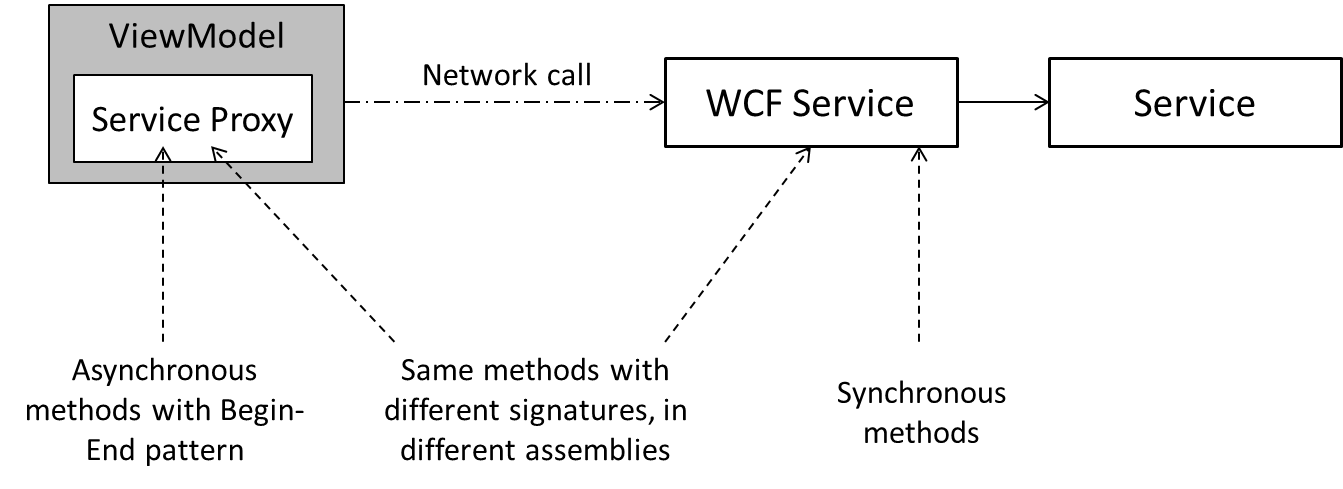
\includegraphics[width=14cm]{figures/fitnesse_start}
\caption{The issues of ViewModel calling exposed server side services}
\label{fig:fitnesse_start}
\end{center}
\end{figure}

There is a need for a architecture which would enable the use of server side services directly from the ViewModels. Also all the asynchronous calls will have to be "translated" to invoke the server side services directly.

The solution to this issue is the creation of wrapper class for the business layer, which can be injected directly to the ViewModel. The wrapper has to take care of the translation of begin - end combination to the call of business layer method and mapping between server side objects and client side objects. The architecture of the functional testing environment is demonstrated on figure \ref{fig:fitnesse_architecture}.

\begin{figure}[h]
\begin{center}
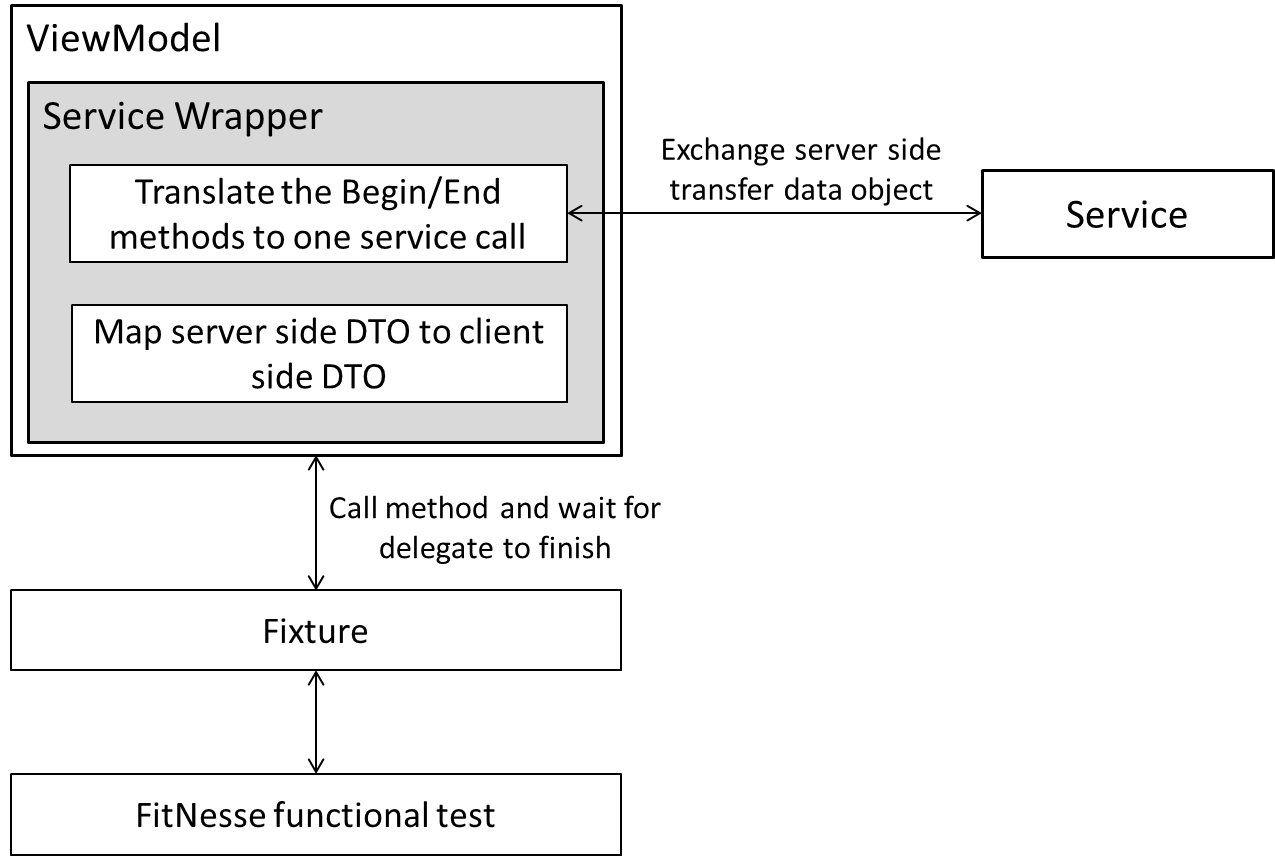
\includegraphics[width=14cm]{figures/fitnesse_architecture}
\caption{Infrastructure for functional testing}
\label{fig:fitnesse_architecture}
\end{center}
\end{figure}

The first step which has to be taken is the translation of "Begin - End" pattern to single method call. This can be achieved by introducing corresponding delegate, because any delegate offers the \textit{BeginInvoke} and \textit{EndInvoke} methods.

\begin{verbatim}
private IService service;

//delegate for a method which takes integer and returns ClientSideDTO
private Func<int, ClientSideDTO> Delegate;

ClientByID = (i) => {
    return Mapper.Map<ServerSideDTO, ClientSideDTO>(service.GetObject(i));
};
            
public IAsyncResult BeginGetObject(int id, AsyncCallback callback, object st)
{
    return Delegate.BeginInvoke(id, callback, st);
}

public ClientSideDTO EndGetObject(IAsyncResult result)
{
    return Delegate.EndInvoke(result);
}
\end{verbatim}

The business layer methods return server side DTO (Data Transfer Object) while the ViewModels work with generated client side DTO objects. These objects are the same, but do not reside in the same assembly, making the implicit conversion impossible. Explicit mapping has to be defined. This can be achieved thanks to auto-mapping libraries such as AutoMapper\footnote{\href{'http://automapper.codeplex.com/'}{AutoMapper} is an open source project generally dedicated to map values of one object to another, common situation which arises for example while converting data base entity object to data transfer object.}. In the above presented snippet, the delegate which calls server side services also uses the \textit{Mapper} class of AutoMapper to make the conversion of server side to client side object.

The last issue comes from the asynchronous nature of the methods in ViewModel. FitNesse has to make assertions after the execution of the operations. However if an assertion follows directly after the \textit{BeginOperation} method, it will be executed before the callback was finished and probably fail.

One option would be to introduce synchronization logic into the callback method. However the callback method is standard part of ViewModel and it would not be wise to increase the complexity of ViewModel for the reason of FitNesse testing.

The possible solution is a combination of signaling and active waiting. The \textit{BeginOperation} method returns \textit{IAsyncResult}. This standard .NET interface contains waiting handle, which signals the end of asynchronous operation. Unfortunately the same signal is send to the callback and starts the execution of the callback.

However all the operations of ViewModel use boolean variable \textit{InProgress} which signals the execution and ending of asynchronous methods. This variable is set to \textit{false} at the end of each \textit{EndOperation} method and thus can be used for active waiting.

Since the active waiting is executed after the signal has come about the termination of asynchronous operation, it is surely after the variable has been set to \textit{true} in the \textit{BeginOperation} method. The use of signal evicts the race conditions which could arise while using only active waiting for \textit{InProgress} variable.

\begin{verbatim}
var customerVM = new CustomerViewModel();

//wrapper instead of real service proxy
customerVM.CustomerService = new CustomerServiceWrapper(_customerServices);
var result = customerVM.GetObject(customer.Id);

//wait for the asynchronous operation to finish
result.AsyncWaitHandle.WaitOne();
result.AsyncWaitHandle.Close();
while (customerVM.InProgress == true) Thread.Sleep(20);

//the customerVM is ready and all service calls have finished
\end{verbatim}

The functional tests (or acceptance tests) prove the correctness of all layers of code. This is a possible advantage over unit tests, while unit tests are isolated to test only one feature. Also the amount of code which has to be written for isolation of unit tests exceeds the amount of code needed for preparation of fixtures. Once the fixtures are prepared business analysts can write the acceptance tests.

\section{Load tests}
Simple usage scenario was defined to obtain metrics about the application deployed to Azure platform.

\begin{itemize}
	\item Client logs into the applications
	\item Client checks the accounts and operations performed on the accounts during last six months. In total the client has 2 accounts, each having 120 categorized transactions.
	\item Client loads to view 5 business partners and personal tags.
	\item 20 client profiles are loaded with tag's repartition, which client can use to make comparison.
\end{itemize}

The test was defined using Fiddler web debugger and StresStimulus plug-in \footnote{Fiddler is web debugger which monitors the HTTP network traffic. Fiddler alone or with plug-ins can be used to analyze the HTTP requests. StressStimulus is a load testing tool available as plug-in for Fiddler. It enables recording and re-execution of HTTP requests. It provides also the possibility to parametrize the requests and define different load strategies}.

The scenario was executed for one client. Figure \ref{tab:metrics_one} provides the obtained metrics. To perform the simulation the network was limited to Dial-Up 56k modem to limit the quality of local connection on the test. Thus the download speed was 56.0 kbit/s and upload speed 33.6 kbit/s.

\begin{table}
\begin{center}
\begin{tabular}{|c|l|}
\hline
Total send bytes & 29792 \\
Total received bytes & 90135 \\
Total HTTP requests & 32 \\
Response time one one request & 1.59 s \\
\hline
\end{tabular}
\end{center}
\caption{Metrics of one execution of typical usage scenario}
\label{tab:metrics_one}
\end{table}

The same scenario was executed again in 60 iterations. During each iteration 5 new clients would ask the same resources. At each second new iteration was executed. After all 60 iterations, the test waited for the requests to finish. Figure \ref{tab:metrics_300} gives the metrics obtained by the execution.

\begin{table}
\begin{center}
\begin{tabular}{|c|l|}
\hline
Number of iterations & 60 \\
Number of users per iteration & 5 \\
Total bytes sent & 1795556 \\
Total bytes received & 5394520 \\
Average response time & 1.85 s \\
Bytes sent per second & 13349 \\
Bytes received per second & 40106 \\
Total number of HTTP requests & 1920 \\
\hline
\end{tabular}
\end{center}
\caption{Metrics obtained by repeated execution of typical use case scenario}
\label{tab:metrics_300}
\end{table}
\chapter{Summary}
This thesis analyzed the current trends in online banking. During the analysis several innovative features were identified such as Personal Finance Management, document digitization and open data management, which will most likely become standard functions offered by the web banking portals.

A set of functional and non-functional requirements was defined. The functional requirements were based mainly on the analysis of innovative functions, but also on the traditional banking functions. The non-functional requirements describe the demands on selected technologies, patterns and architectures.

After the requirements were defined a technical solution was provided which solves most of the issues identified in the first part. This solution is build upon .NET technology stack and uses several open source libraries and components to implement the defined system. Since Cloud platforms are gaining in popularity and usability, the solution was designed to be deploy-able to Cloud platform. Azure platform was chosen to fit the .NET nature of the solution.

This thesis has shown, that it is possible to build innovative system using open source or self-developed components. Features such as authentication using face recognition, payment categorization or implementation of electronic vault were defined and successfully developed. The solution has a service oriented architecture. All business layer functions are exposed as stateless services. This assures that the solution can in the future support any type of front-end client application.

Universal approach was described in this thesis which gives the possibility to reuse the majority of the code in the presentation layer on Windows Phone 7 and Silverlight platforms, thanks to Model-View-ViewModel pattern.

Modularity of the application was one of the non-functional requirements. The solution was designed to allow future replacements or improvements of individual modules. It should not be complicated to replace individual components by new ones, such as provide new image processing library for face authentication or completely change the data access layer.

Special emphasis has been put on the testability of the solution. The solution was designed to allow testability of all of the parts and application modules. Infrastructure was build to allow the definition of functional tests by non-developers.

Even though, that several innovative features were successfully implemented, not all the functions defined in the initial analyzes were developed. There is still a place to continue this work in two directions.

First direction is the development of innovative features identified during the analysis which were not implemented. Since the web in general changes in fast pace, new innovative ideas will also emerge.

Second direction is the improvement of the developed parts, such as new categorization engine based on different machine learning algorithm or change of the algorithm used for face authentication.

% originally following specification for bibliography formating was used
%\bibliographystyle{abbrv}
\bibliographystyle{plainnat}

%\bibliographystyle{csplainnat}

%bibliographystyle{plain}
%\bibliographystyle{psc}
{
%JZ: 11.12.2008 Kdo chce mit v techto ukazkovych odkazech take odkaz na CSTeX:
%\def\CS{$\cal C\kern-0.1667em\lower.5ex\hbox{$\cal S$}\kern-0.075em $}
\bibliography{reference}
}

\appendix

\chapter{Technology choices}
During the design and implementation of the application several technology choices have to be made. This chapter briefly justifies and summarizes the selected frameworks and technologies.
\section{Communication and integration}
\label{tech:wcf}
The design of the communication layer is based on Windows Communication Foundation (WCF), which is standard part of .NET framework. Unlike in the Java ecosystem, where there are several communication frameworks (such as Apache Axis and Apache CXF), in .NET Windows Communication Framework is the preferred choice and usually no alternatives are taken into account. WCF provides the developer with the flexibility of choosing transportation protocol (TCP, HTTP, MSMQ) as well as the transportation format (XML, JSON, Binnary).

One service can expose several Endpoints (URIs). Each Endpoint can be configured to use different Binding. Bindings can have different transportation protocols and format options. The same services can be thus exposed using different protocols and formats. In our application we can use this advantage and expose different endpoints for different clients. This is crucial for platform independent applications.

\section{Data access}
\label{tech:data}
The most important part of the Data Access layer is the framework used for Object Relational Mapping (ORM). There are currently two major ORM frameworks in .NET:  NHibernate and Entity Framework. Both provide similar ORM features such as: code only approach, lazy loading, use of Poor old CLR objects(POCO) as persistence classes and integration of Language Integrated Query (LINQ).

Entity Framework 4.0 has brought a lot of improvement to its previous version (named Entity Framework 1.0) which did not provide above mentioned functions and nowadays Entity Framework is comparable to NHibernate.

NHibernate has still several advantages among these it's better ability to process batch treatment and also the fact that as an open source product it can be customized. There are also several extension projects (NHibernate Shards, NHibernate Search, Fluent NHibernate) which build up on NHibernate. Entity Framework provides build-in integration with Visual Studio, however thanks to the open-source nature of NHibernate similar integration tools were build also for NHibernate\footnote{Mindscape has released free edition of NHibernate Designer}.

\subsection{Definition of database mapping}
NHibernate uses its XML based HBM format to define the mappings between entities and POCOs. While the separation of code and configuration in XML can be seen as advantageous approach it gets complicated once the XML configuration files are larger and once we are introducing changes into the POCOs. The XML is not checked upon the compilation, so potential errors can be detected at run-time only and are generally hard to localize.

As a solution to this issue Fluent NHibernate allows the developer to define the mappings in strongly-typed C\#, which practically eliminates these issues. If there is an error in configuration, it will be most likely discovered during the compilation (or sooner thanks to Visual Studio type checking). Currently Fluent provides almost full compatibility with HBM files.

\subsection{Data generation}
While developing data based applications, it is important to have testing data since the beginning of the implementation phase. AutoPoco is a simple framework which allows generation of POCOs (Plain Old CLR Objects) with meaningful values. Autopoco provides easy way to generate the starting data. It also provides several build-in sources for common properties which are stored in databases such as phone numbers, birth dates, names and credit card numbers. The framework is also extensible and allows developers to create own data sources, for specific custom properties.

\section{Application composition}
\label{tech:di}
There are two design patterns (or approaches) which are very often used in order to compose the application from several modules: Dependency Injection and Aspect Oriented Programming.

Dependency Injection is used to assemble complex system from existing blocks. There are several Dependency Injection containers available for .NET framework: Spring.NET, CastleWinsdor, StructureMap, AutoFac, Ninject, Unity (by Microsoft), LinFu.

Aspect Oriented Programming allows developers to separate cross-cutting concerns from the applications blocks. This is usually done by injecting code into object's existing methods.
In the .NET ecosystem, there are two ways used to implement aspect oriented programming: Proxy based AOP and IL Weaving based AOP.

Proxy based AOP is easily achieved by wrapping targeted object by a proxy class. Than it is easy to intercept the calls to the target object by the proxy class and call the code, which should be injected. 
The majority of Dependency Injection containers use proxy classes and therefor most of them offer also AOP. (Spring.NET, CastleWinsdor).

IL Weawing is an expression for injection of Intermediate Language (IL) code after compile time before the generation of byte-code.

There are two frameworks which provide AOP through IL Weaving: PostSharp and LinFu. PostSharp offers a commercial license. LinFu is an open-source project under LGPL license which covers both Dependency Injection and AOP.

Spring.NET has been chosen because of it's maturity, the fact that it is well documented, works well with NHibernate and allows both Aspect Oriented Programming as well as Dependency Injection. One of the disadvantages of Spring.NET is the XML configuration which can become too large to maintain and again is not checked during compilation and may be a source of errors. 

There are other frameworks, which us C\# as the language to configure the AOP or Dependency Injection. For instance PostSharp makes use of attributes and Ninject or StructureMap use strongly typed classes to configure the Dependency Injection container.

\section{Security}
The security of the application is based on Forms Authentication being the standard way of securing .NET web applications. Forms Authentication scheme works by issuing a token to user the first time that he authenticates. User can be authenticated against database or any other information source.

This token in the form of cookie is added to the response which follows the authentication request. This way the cookie is added to the next request by the same client. Forms Authentication than takes care of revoking the cookie (after demanded time)  as well as of checking the cookie in each requests.

Forms Authentication works automatically with browser based clients, when used from different clients, some additional work on the client has to be done in order to add the authentication cookie to each request.
 
DotNetOpenAuth library was used in order to enable the support of OAuth protocol.

\section{Unit testing}
\label{tech:unit}
Visual Studio provides standard unit testing framework called MsTest, therefor there is no need for external libraries. Thus this section discusses the options which have been chosen to isolate unit tests from the rest of the application code.

\subsection{Isolation of unit tests}
\label{tech:isolation}
In order to write efficient unit tests, the tests have to be isolated from the rest of application code. To achieve that two conditions have to be fulfilled.
\begin{itemize}
	\item  Each module has to be defined by interfaces.
	\item  Isolation framework should be used to provide simple implementations for defined interfaces.
\end{itemize}

The activity of replacing existing interface by implementation simple enough just to fulfill the needs of the test is called "mocking". There are several Mocking frameworks available: NMock, EasyMock, Moq, JustMock (commercial), TypeMock (comercial), RhinoMocks, NSubstitute, FakeItEasy and Moles.

For this application RhinoMocks and Moles were chosen. Moles are used only for parametrized unit testing and are discussed in \ref{tech:moles}.
RhinoMocks is an open source framework, easy to be used with active community. It was created by Ayende Rahien, the author of NHibernate. It works also with Silverlight.

\section{Presentation layer}
The choice of presentation layer was already part of the assignment. OCTO Technology wanted to use Silverlight 4. Putting aside that the choice was already done, here is a brief comparison of Silverlight and other alternative presented by the combination of HTML 5 and JavaScript.

\subsection{Characteristics of Silverlight}
Here is a list of characteristics which can be seen as advantages.
\begin{itemize}
	\item Intended to develop Rich Internet Applications.
	\item Supports separation of the view and the logging using the MVVM pattern.
	\item Possibility to use declarative language (XAML) to design user interface and imperative language to define the application logic.
	\item Data visualization support using open source Silverlight Toolkit (charts, line series)
	\item Re-usability of code on .NET compliant platform.
	\item Possibility to access audio and video devices on client side.
	\item Plug-in based technology. Requires the plug-in to be run inside the browser. The plug-in is not available for all possible combinations of platform and browser. This lowers the availability of the developed application and brings also higher requirements on hardware.
	\item Standard web features are missing such as navigation.
	\item Limited testability. Silverlight can not be tested with traditional functional testing frameworks such as Selenium. On the other hand, when the MVVM pattern is implied, the ViewModels can be tested as simple classes, using traditional Unit Testing technologies.
\end{itemize}

\subsection{Characteristics of HTML 5 / JavaScript combination}
\begin{itemize}
	\item  No plug-in needed, HTML 5 is supported on the majority of the current browsers.
	\item  Naturally comes with web standard features: navigation, bookmarking.
	\item  Developers has to handle the "all browsers compatibility" issue.
	\item  Compared to C\# JavaScript is dynamic language, not compiled before the execution. This may be seen as advantage and disadvantage.
\end{itemize}

The decision between Silverlight and HTML depends on the project type. For line-of-business applications where the platforms used to run the applications are know before (and conform to Silverlight), Silverlight is a good choice.

On the other hand, for widely open internet applications, the combination of HTML 5 and JavaScript will be the right choice assuring the availability of the application for everyone, regardless the platform. Currently HTML 5 supports almost all features provided by Silverlight.

It is good to mention, that Silverlight as platform is based on the subset of Windows Presentation Framework. Windows Phone 7 platform was based on Silverlight and the new application runtime for Windows 8 (WinRT), is based on the same language and architecture. Thus the code ones written for Silverlight could be later used in Windows 8, Windows 7 and XBox device and might be a good solution for companies which invest heavily in Microsoft technologies.
\chapter{Technology details}
\section{Message Authentication}
\label{tech:azure_blob_storage}
Shared Access Signature scheme proposed by Azure Blob Storage is marketing name used for Message Authentication Code, standard term in cryptography, describing short piece of information which authenticates a message. The same mechanism is used as well in Amazon S3 (offer concurrent to Azure Blob Storage) but here it is called "Expiring URL".

Shared Access Signature is generated using standard HMAC (Hash-base Message Authentication Code) algorithm. HMAC algorithms use one of the existing hash functions in combination with the secret key to generate the MAC value.

Azure Blob storage uses the HMACSHA256 function, which as the name says, makes use of 256-bit SHA function and has the following definition (where “|” represents concatenation):

\begin{equation}
HMACSHA256 (key, data) = sha256(sha256(data|key)|key)
\end{equation}

The hash is applied two times during the process in order to disable attacks which were successful on previously simpler variants of the function which had used just hashed combination of data and key\cite{wiki:hmac}. The key is simply the Azure Blob Storage access key however the data is the combination of the following:

\begin{itemize}
	\item Identification of resource which should be accessed (container or blob)
	\item Time stamp – specifying the expiration date
	\item Permissions which will be given to access the resource
\end{itemize}

The same data is added to the request, so when the server receives the request, it performs the same calculation of the HMAC value to verify the Shared Access Signature. That is possible because the server is in possession of the access key.

\section{Face recognition methods and algorithms}
\label{tech:face_recognition}
There following is a short list of two dimensional face recognition techniques\cite{Patil10}.
\begin{description}
	\item [Statistical methods] Methods which use statistics do define different ways to measure the distance between two images. In other words they try to find a way to define how similar two faces are to each other. There are several methods which fall into this group containing Linear Discriminant Analysis, Independent Component Analysis, Principal Component Analysis.
	\item [Gabor Filters] Filters commonly used in image processing, that have a capability to capture important visual features. These filters are able to locate the important features in the image such eyes, nose or mouth. This method can be combined with the previously mentioned analytical methods to obtain better results.
	\item [Neural Networks] Neural Networks are simulating the behavior of human brain to perform machine learning tasks such as classification or prediction. Neural Network is a set of interconnected nodes. The edges which are between the nodes are weighted so the information which travels between two nodes can be amplified. The information travels from set of input nodes, across a set of hidden nodes to a set of output nodes. The developer has to invent a way to encode the input (in this case an image) to a set of input nodes and decode the output (in this case a label identifying the person) from the set of output points.
	Commonly used method is to take one node for each pixel in the image on the input side of the network and one node for each person in the database on the output side.
\end{description}

\section{Details of PCA algorithm}
\label{tech:eigenface}
The general purpose of PCA algorithm is to reduce the large dimensionality of the data space to smaller dimensionality of feature space, which can still be used to describe the data.

As the set of features used to describe the object, the first several eigenvectors and eigenvalues of covariance matrix are used. Eigenfaces are graphical representation of eigenvectors and can be visualized as images.

It has been shown, that the the eigenvectors associated with the largest eigenvalues are the ones that reflect the greatest variance in the image. Roughly 90\% of the total variance can be contained in the first 5\% to 10\% of the dimensions \cite{Kyungnam01}.

Each image can be than projected on M dimensions (where M is the chosen number of eigenvectors). Thus the number of dimensions is reduced from the number of pixels onto the number of eigenvectors. Each image is then expressed as a vector of size M. The distance between two images can be defined as euclidean distance between these two vectors.

\section{Haar Cascade face detection}
\label{tech:haarcascade}
Method which was introduced by Viola and Jones \cite{Viola01}. The Haar-like features rather than using the intensity values of a pixel, use the change in contrast values between adjacent rectangular groups of pixels \cite{Wilson06}. The sub-arrays of the image are scanned and the intensities of the pixels of each sub-array are added in order to determine the features depicting edges, lines or center-surrounds.

To learn the Haar-cascade classifier a set of negative (without a face) and positive (containing a human face) images has to be provided. The classifier works in a cascade. That means, that several simple classifiers are sequentially used to set image as positive or negative. The image is set as positive if it passes all the cascade.

OpenCV library already contains both: the algorithm to build and learn the classifier from arbitrary images and also built-in classifier for detecting human faces \cite{opencv:facedetection}.

\section{Parametrized unit testing}
\label{tech:parametrized_testing}

Parametrized unit testing is used to simplify the generation of unit tests. Pex framework is used analyze the code under the test and generate inputs for unit tests in order to exercise all branches of tested code.

Pex internally uses algebraic solver Z3 from Microsoft Research to determine the values of all the variables that may affect the branching to analyze all branches.

For each branch in tested code, Pex builds  a formula, that represents the condition under which this branch may be reached. This formula is handed to Z3 algebraic solver, which uses decision formulas to decide the values of variable to reach the branch \cite{Tillman08}.

By default Pex analysis the code of all of the loaded assemblies to determine the right inputs. During the analysis Pex enters event into the isolation framework and tries to define such input variables that it would cover all the branches not only inside the tested code, but also inside the isolation framework.

For that reason it is recommended to use Moles \ref{tech:moles} isolation framework, which is designed in order to be used with Pex.

\section{Moles stubbing framework}
\label{tech:moles}
Moles is a stubbing framework build by Microsoft Research to work well together with Pex. Moles works in a similar way as other frameworks, letting the developer to define return objects for executed methods. On the other hand, Moles generates the stubs of interfaces during the compilation, while other frameworks (as for example Rhino.Mocks) are able to create the stubs at run-time.

Second advantage of Moles, which is not connected only to parametrized testing, is the fact, that it is able to substitute any method by delegate including static methods and methods inside .NET framework. This is particularly useful in cases when the code relies on static methods from .NET framework. Typical example of this situation is the usage of \textit{DateTime.Now} or \textit{Guid.NewGuid}. These methods are often called in business layers of applications and complicate the testing of the business layer.

Using Moles the delegate which will be invoked on the particular method or property can be set. The following snippet shows the definition of static .NET class \textit{Guid} which resides directly inside the \textit{System} assembly.
\begin{verbatim}
public static class Guid { 
  public static Guid NewGuid();
}	
\end{verbatim}
To change the behavior of that class a mock is defines before the compilation by Moles framework.
\begin{verbatim}
public class MGuid { 
  public static 
    Func<Guid> NewGuid { set; get;}
}
\end{verbatim}
By assigning a delegate to this mock, the developer can specify the return value of the function. In the following assembly lambda expression is inserted instead of delegate.
\begin{verbatim}
MGuid.NewGuid = () => new Guid("64d80a10-4f21-4acb-9d3d-0332e68c4394");
\end{verbatim}
In order to execute code assigned to the delegate inside the mock instead of the original code of the method just in time injection is performed by the Moles hosting environment, which checks whether any delegate was defined and executes the delegate if it was the case.
\begin{verbatim}
public static class Guid { 
  public static Guid NewGuid() {
  
    //begin - injected at runtime
    if (MGuid.NewGuid != null)
      return MGuid.NewGuid();
    
    //end - injected at runtime
    ...original code...
  }
}
\end{verbatim}

\section{Code verification}
Design by contract is software design approach, which implies that developers define clear interfaces for each software component, specifying its exact behavior. The interfaces are defined by contracts and extend the possibilities of code verification and validation.

The term "Design by Contract" was first used by Bertrand Meyer, who made it part of Eiffel programming language \cite{Meyer92}.

Code Contracts is a language agnostic framework which enables the "Design by Contract" approach \cite{ContractsManual} by allowing the programmer to define three types of conditions for each method:
\begin{description}
	\item [Pre-condition] States in what forms the arguments of the method should be.
	\item [Post-condition] States what forms the outputs of the method will have.
	\item [Invariants] Conditions which will always be true during the execution of the method.
\end{description}

These conditions can be later verified by two types of checks:

\begin{description}
	\item  [Static checking] Checking procedure evaluated at the compilation time. At this time the compiler does not know what will be the values passed as arguments to the methods, but from the execution tree it can determine which method calls might potentially be evoked with non-compliant parameters.
	\item  [Runtime checking] The code contracts are compiled as conditions directly into .NET byte-code. This allows the program to avoid writing conditions manually inside the method bodies.
\end{description}

Note that Code Contracts are not language feature. They are composed of class library and the checking tools which are available as plug-ins for Visual Studio.
\chapter{Description of the projects in the solution}
The solution is composed of several interconnected projects. Diagrams \ref{fig:dependency_server_side} and \ref{fig:dependency_client_side} depict the dependencies between the projects. Here follows the description of each project.
\begin{description}
	\item[Octo.Bank.Core] Project which defines all interfaces which build the application.
	\item[Octo.Bank.CoreDomain] The class model of the application domain. The class model is depicted on figures \ref{fig:domain_model_1} and \ref{fig:domain_model_2}.
	\item[Octo.Bank.DataAccess] Implementation of the interfaces which mediate the access to database.
	\item[Octo.Bank.DbTool] Console application for generation of database schema and initial data.
	\item[Octo.Bank.Dto] Data transfer objects, which are serialized into XML, JSON, or proprietary binary format.
	\item[Octo.Bank.Services] Implementation of the business layer services.
	\item[External.ConsumerApp] Web implementation of OAuth consumer for testing.
	\item[ml] The solution of machine.codeplex.com library, with implemented Naive Bayes classification.
	\item[ml.Tests] Unit tests for the machine.codeplex.com library.
	\item [Octo.Bank.Mobile] Windows Phone 7 application.
	\item [Octo.Bank.Mobile.MVVM] MVVM framework prepared for compilation on Windows Phone 7 platform.
	\item [Octo.Bank.Mobile.ViewModels] ViewModels linked from Silverlight project, prepared for compilation on Windows Phone 7.
	\item [Octo.Bank.ParametrizedTests] Parametrized unit tests generated using Pex framework.
	\item [Octo.Bank.TestFixtures] Dynamic library, containing fixture classes which are invoked by FitNesse functional test framework.
	\item [Octo.Bank.Tests] Standard unit tests for data access and business service layer.
	\item [Octo.Bank.Web.Ria.UnitTests] Unit tests for ViewModels classes.
	\item [Octo.Bank.MVVM] Silverlight 4 version of the MVVM framework.
	\item [Octo.Bank.Web] Main web application, hosting the Silverlight package and WCF services.
	\item [Octo.Bank.Web.Ria] Silverlight project, containing also the ViewModels of the application.
	\item [Octo.Bank.Web.Ria.Components] Silverlight user controls, which might serve also in other applications (such as event calendar).
	\item [Octo.Bank.CloudService] Project used for the deployment to Azure platform.
	\item [Octo.Bank.Models] Project containing dependency graphs.
	\item [Octo.Bank.PortableServices] Proxy classes for communication services compiled as portable class library. This project is referenced from Windows Phone 7 and Silverlight projects.
\end{description}

\chapter{UML Diagrams}

\begin{figure}[h]
\begin{center}
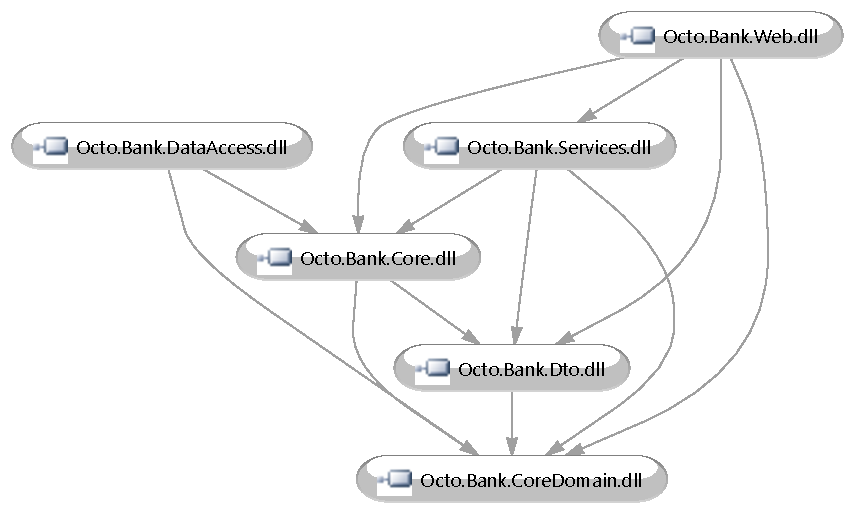
\includegraphics[width=14cm]{figures/dependency_server_side}
\caption{Dependency diagram of the back-end part of the application}
\label{fig:dependency_server_side}
\end{center}
\end{figure}

\begin{figure}[h]
\begin{center}
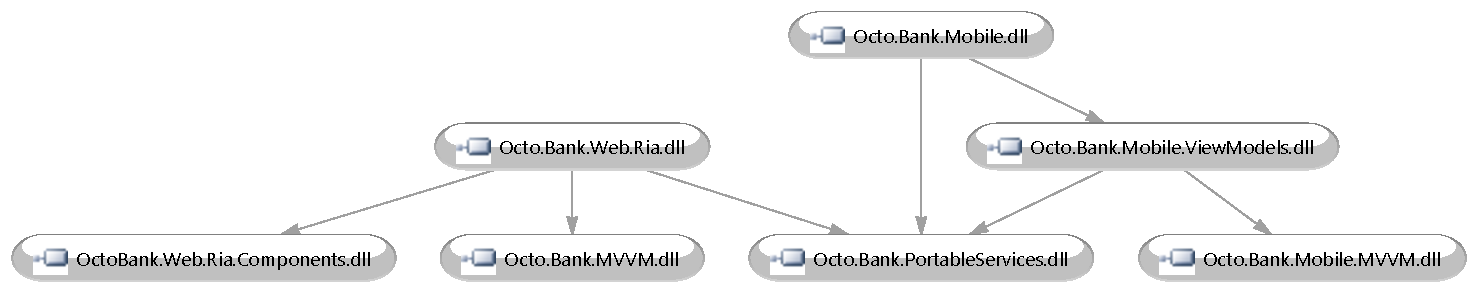
\includegraphics[width=14cm]{figures/dependency_client_side}
\caption{Dependency diagram of the client-side part of the application}
\label{fig:dependency_client_side}
\end{center}
\end{figure}

\begin{figure}[h]
\begin{center}
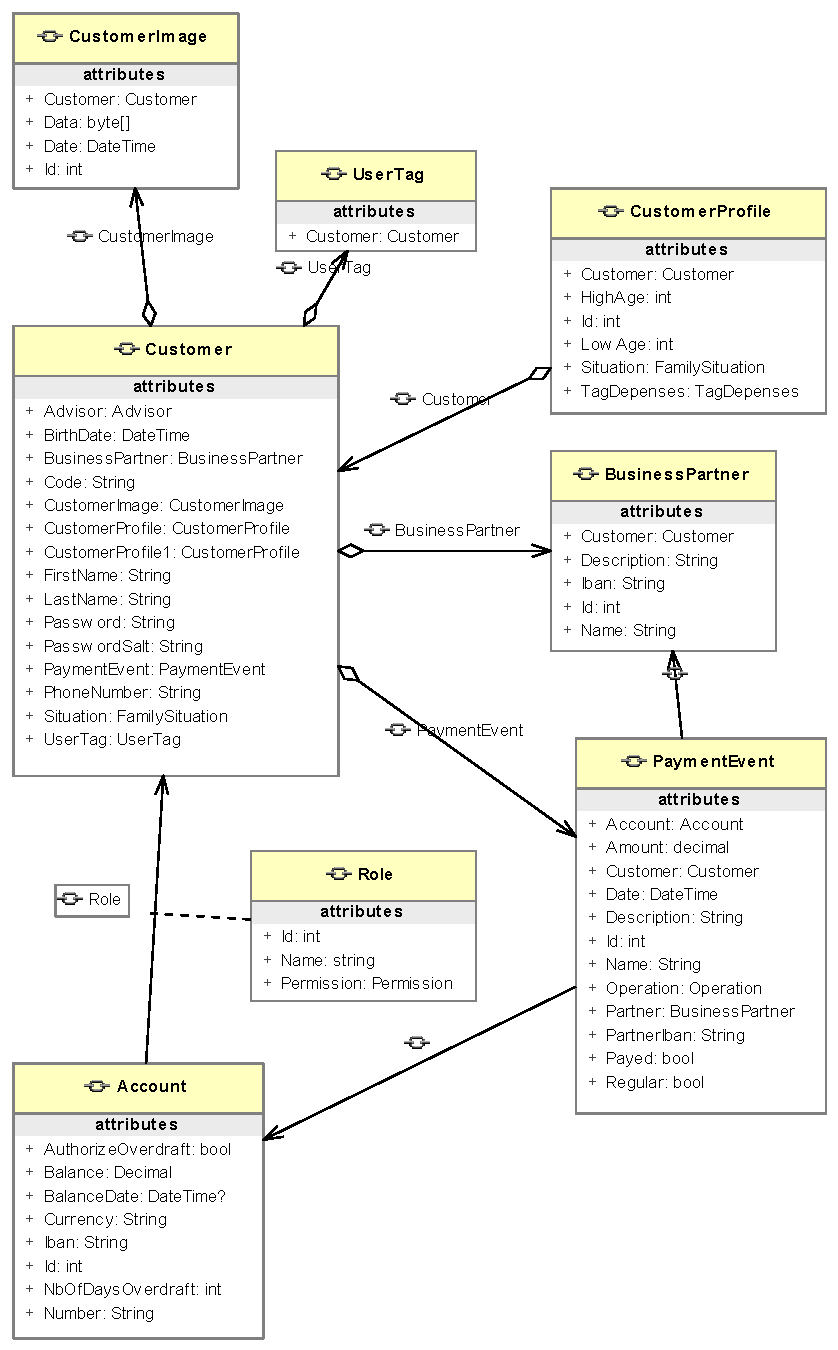
\includegraphics[width=14cm]{figures/customer_oriented}
\caption{Domain model concentrated around the \textit{Customer} entity}
\label{fig:domain_model_1}
\end{center}
\end{figure}

\begin{figure}[h]
\begin{center}
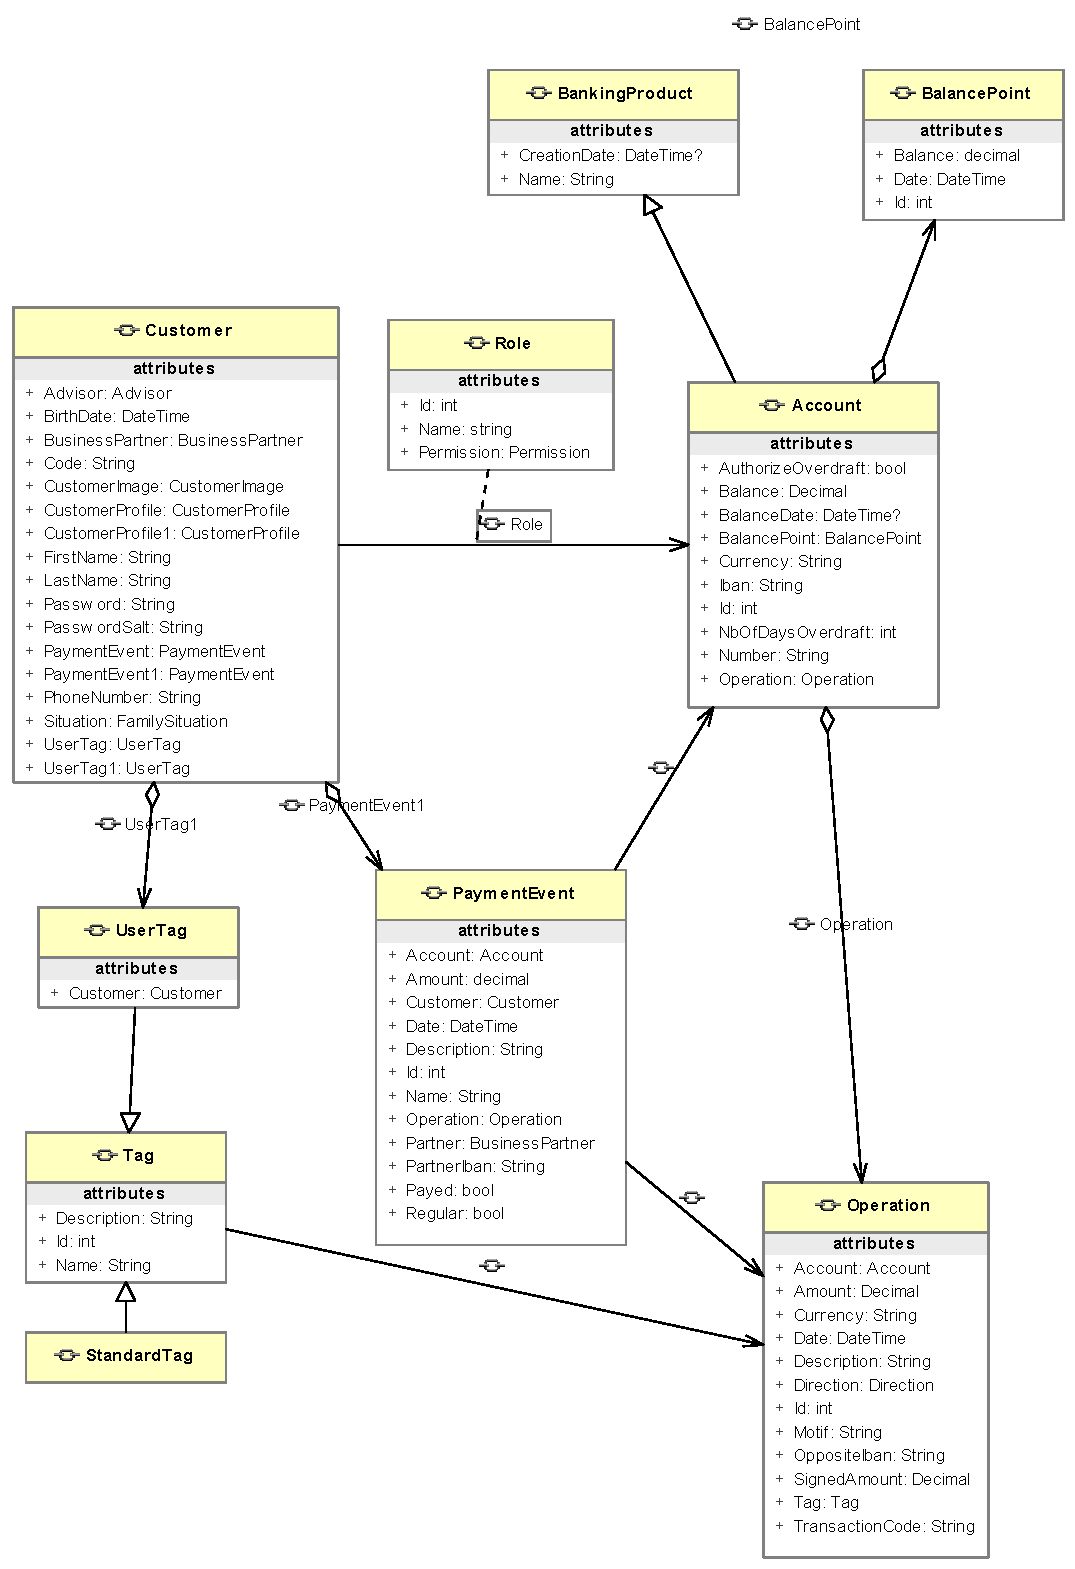
\includegraphics[width=14cm]{figures/operation_oriented}
\caption{Domain model concentrated around the \textit{Operation} entity}
\label{fig:domain_model_2}
\end{center}
\end{figure}

\begin{figure}[h]
\begin{center}
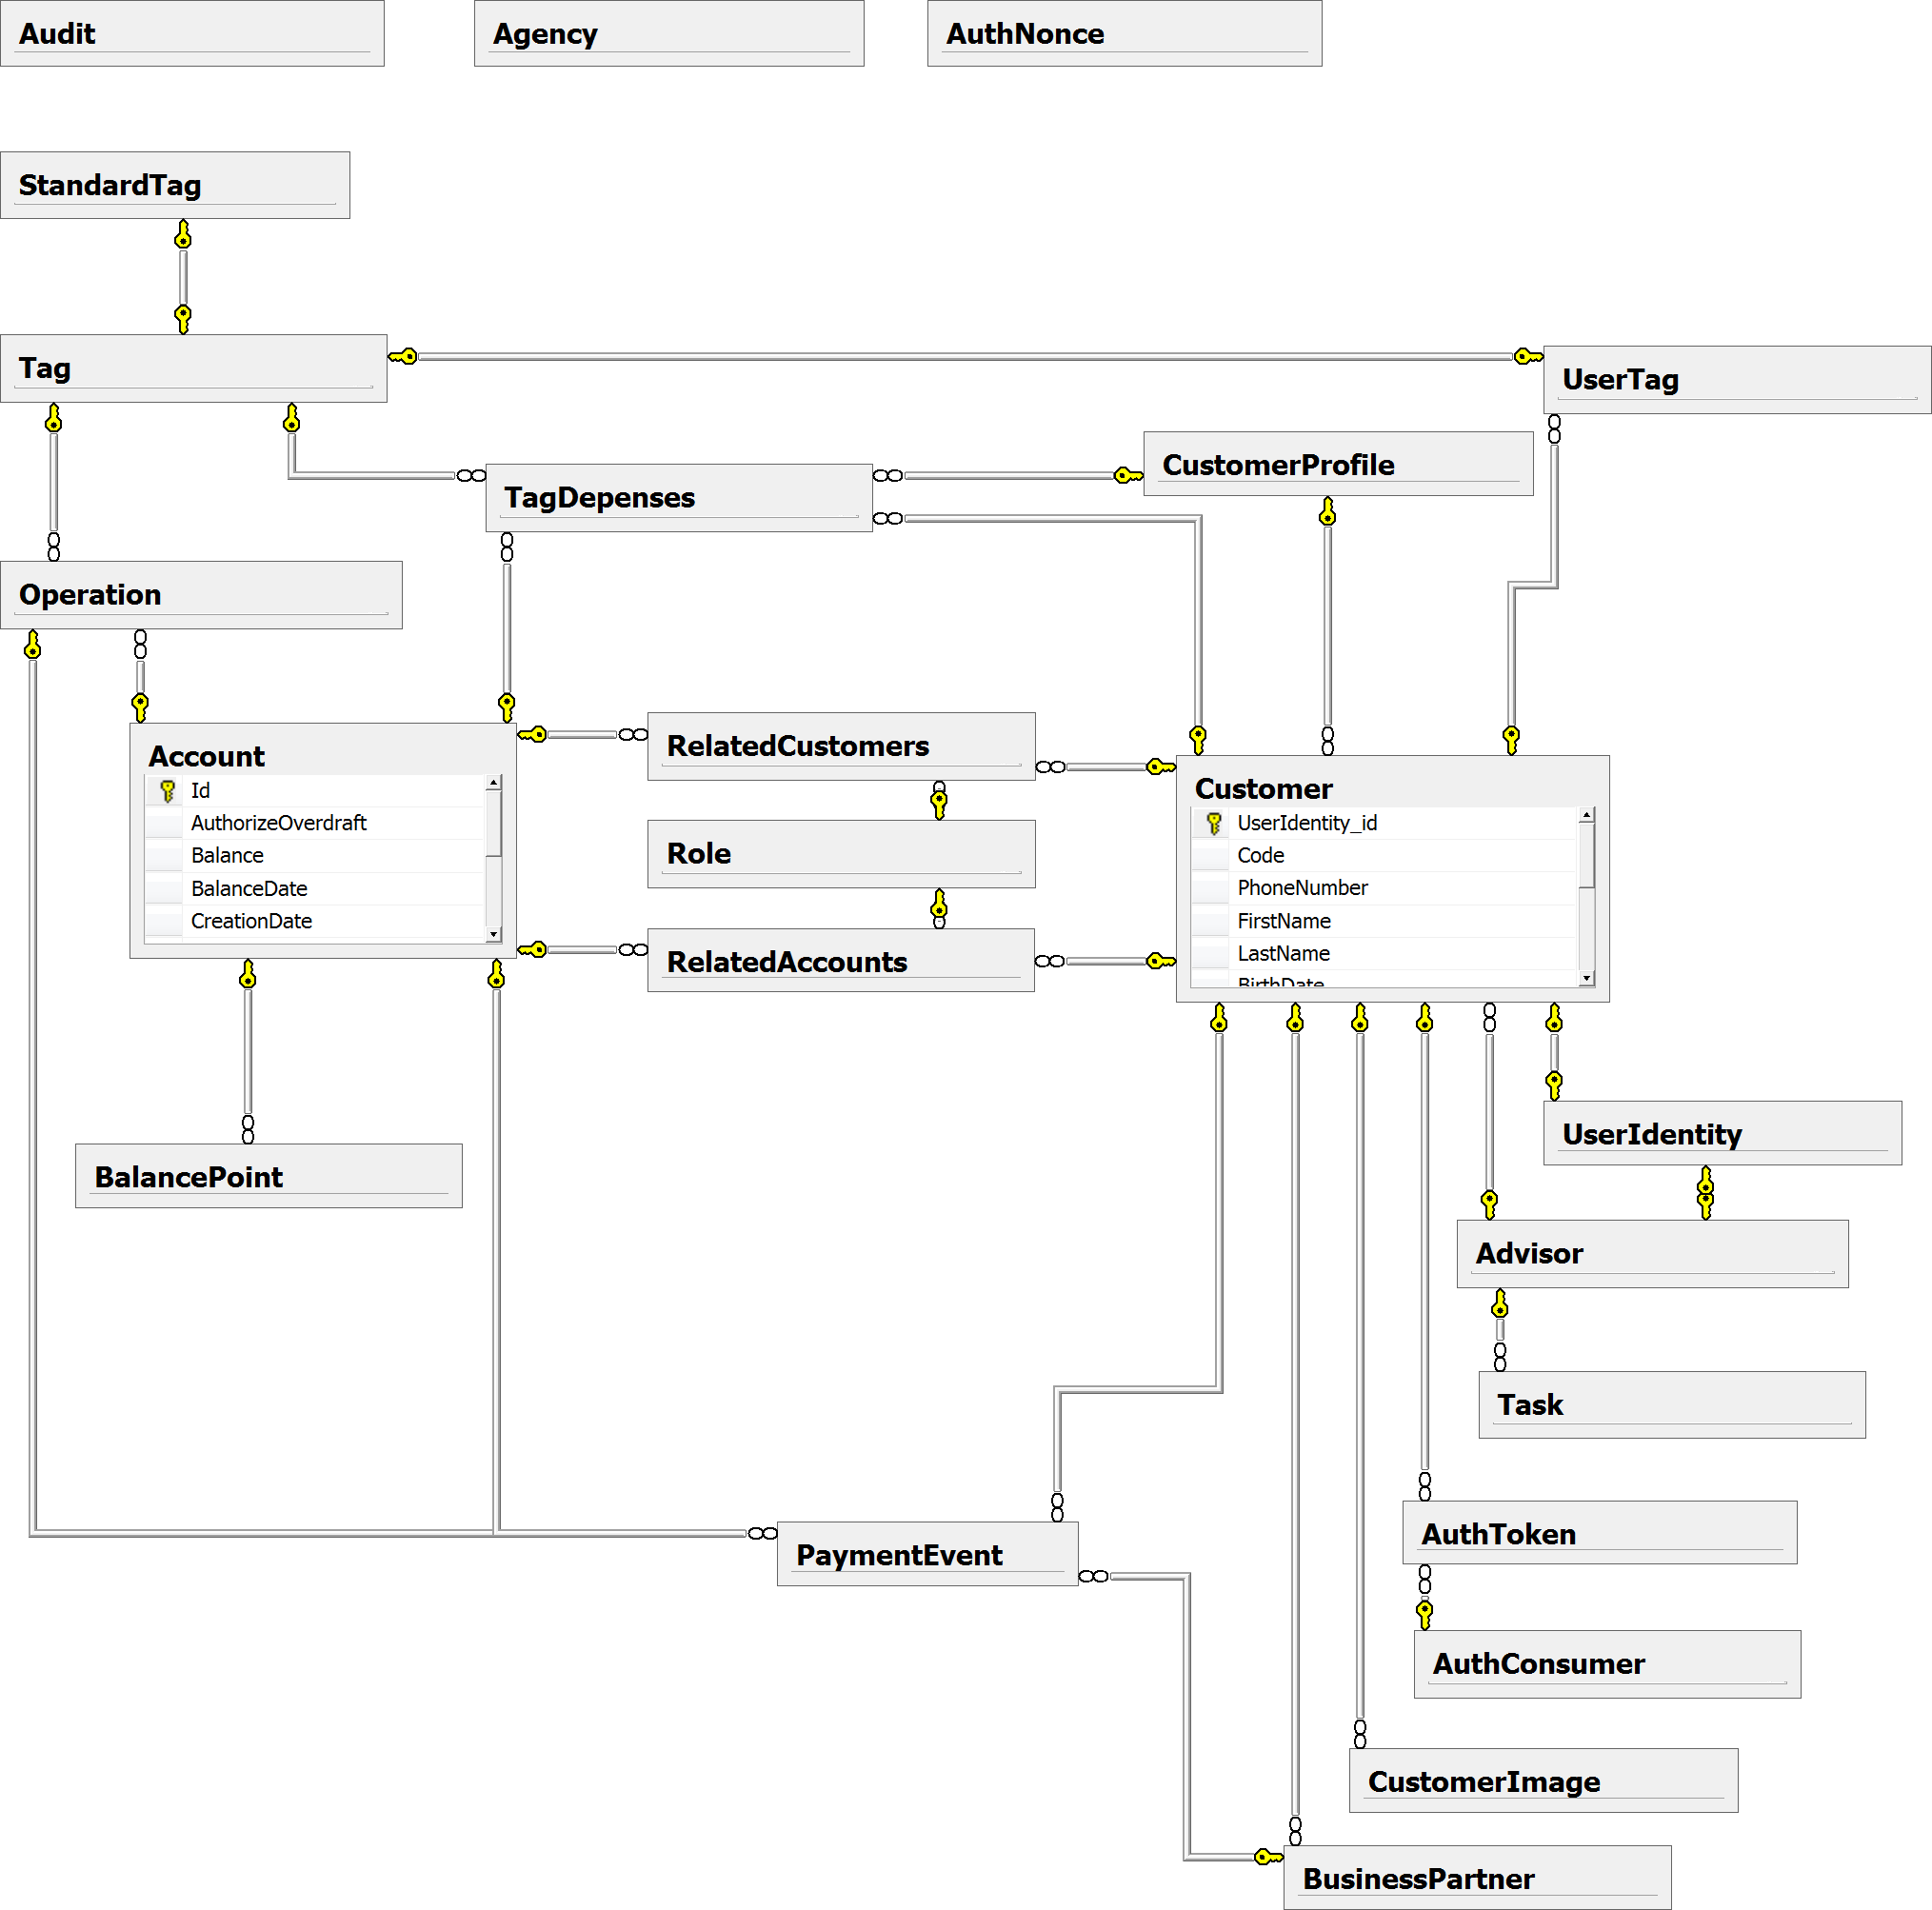
\includegraphics[width=14cm]{figures/db_diagram_all}
\caption{Entity relationship model of the database}
\label{fig:er_model}
\end{center}
\end{figure}

\chapter{List of used abbreviations}

\begin{description}
\item [AJAX] Asynchronous JavaScript and XML
\item [API] Application Programming Interface
\item [BLOB] Binary Large Object
\item[CBS] Core Banking System
\item [CLR] Common Language Runtime
\item [CSV] Comma Separated Values
\item[DES] Data Encryption Standard
\item [DLL] Dynamic Link Library
\item[DTO] Data Transfer Object
\item[ESB] Enterprise Service Bus.
\item [HMAC] Hash-based Message Authentication Code
\item[HTTP] Hypertext Transfer Protocol
\item [IIS] Internet Information Server
\item [IL] Intermediate Language
\item[JSON] JavaScript Object Notation
\item[LINQ] Language Integrated Query
\item [MSMQ] Microsoft Message Queuing
\item [MVC] Model View Controller
\item [MVVM] Model View ViewModel
\item[OCR] Optical character recognition
\item[ORM] Object Relational Mapping
\item[PCA] Principal Component Analysis
\item[PDF] Portable Document Format
\item[PFM] Personal Finance Management
\item[RIA] Rich Internet Application
\item[REST] Representational State Transfer
\item[SHA] Secure Hash Algorithm
\item[SOAP] Simple Object Access Protocol
\item [SSL] Secure Sockets Layer
\item [TCP] Transmission Control Protocol
\item[WCF] Windows Communication Foundation
\item[XML] Extensible Markup Language
\end{description}





\chapter{Content of the attached CD}
\begin{verbatim}
--> readme.txt - Explications and descriptions to run and build the solution
--> text - The text of the diploma thesis
--> src - The source codes
 |--> Libraries - External DLL files referenced in the solution
 |--> Octo.Bank.sln - Solution file which can be opened using Visual Studio
 |--> Octo.Bank.[Project] - Different projects which are part of the solution
\end{verbatim}

\end{document}